%%%%%%%%%%%%%%%%%%%%%%%%%%%%%%%%%%%%%%%%%%%%%%%%%%%%%%%%
%%%%%%%%%%%%%%%%%%%%%%%%%%%%%%%%%%%%%%%%%%%%%%%%%%%%%%%%
%%			            Capitulo 4					  %%
%%%%%%%%%%%%%%%%%%%%%%%%%%%%%%%%%%%%%%%%%%%%%%%%%%%%%%%%
%%%%%%%%%%%%%%%%%%%%%%%%%%%%%%%%%%%%%%%%%%%%%%%%%%%%%%%%
\chapter{Resultados} \label{cap4}



\newpage

%%%%%%%%%%%%%%%%%%%%%%%%%%%%%%%%%%%%%%%%%%%%%%%%%%%%%%%
%		            	Seccion          			  %
%%%%%%%%%%%%%%%%%%%%%%%%%%%%%%%%%%%%%%%%%%%%%%%%%%%%%%%
\section{Lectura y multiplexado de eventos teclado - ratón con ``Reactor''} \label{s4_1}

%%%%%%%%%%%%%%%%%%%%% Subsección %%%%%%%%%%%%%%%%%%%%%
\subsection{Instalación de ``Reactor''} \label{s4_1_1}

La biblioteca ``Reactor’’ es una biblioteca de software libre que ha sido pensada para el uso académico en Trabajos de Fin de Grado impartidos en la Universidad de Castilla-La Mancha. Se encuentra disposnible respositorio de su desarrollador, Francisco Moya: ``http:\textbackslash \textbackslash github.com/\\FranciscoMoya/rpi-src’’. Puede descargarse directamente o si se dispone de un sistema de control de versiones GIT\footnote{Véase la sección 1,5.}, se puede clonar el repositorio: \\

\begin{bashcode}
$ cd Desktop
$ clone http:\\github.com/FranciscoMoya/rpi-src
\end{bashcode}

Accediendo a la ruta ``Desktop/rpi-src/c/reactor/reactor’’ se observan aquellos archivos ``.c’’ y cabecera o ``.h’’ necesarios para compilar aquellos programas que hagan uso de esta biblioteca.

Algunas pruebas que se realizan con ``Reactor’’ necesitan, a su vez, archivos de otra biblioteca llamada ``WiringPi’’. Para comprobar si está instalada en el sistema, se teclea en el terminal la orden:\\

\begin{bashcode}
$ gpio -v
\end{bashcode}

Si aparece la versión y demás contenido informativo, se concluye que la librería está instalada. Si no es así y si se dispone de GIT, basta con clonar de nuevo el repositorio WiringPi: \\

\begin{bashcode}
$ git clone git://git.drogon.net/wiringPi
\end{bashcode}

Para instalarlo, se introduce lo siguiente en el terminal:\\

\begin{bashcode}
$ cd wiringPi
$ ./build
\end{bashcode}

El script ``build’’ realiza la compilación y la instalación de WiringPi. 
Una vez hecho esto, se procede a contruir la biblioteca ``Reactor'' con todos los archivos de ``Desktop/rpi-src/c/reactor/reactor’’: \\

\begin{bashcode}
$ cd Desktop/rpi-src/c/reactor
$ make
\end{bashcode}

La última orden crea la biblioteca ``libreactor.a’’ sin problemas ya que se detecta perfectamente el archivo cabecera ``wiringPi.h’’ de la biblioteca anterior la cual, ha sido previamente instalada.


%%%%%%%%%%%%%%%%%%%%% Subsección %%%%%%%%%%%%%%%%%%%%%
\subsection{Resultados de la lectura y multiplexado de eventos} \label{s4_1_2}

Como ya se ha descrito en la sección 3.1.3.3, este programa realiza la apertura de las interfaces ``Hidraw’’ de entrada/salida de los dispositivos HID para acceder a los eventos enviados por el ratón y el teclado conocidos como los clientes de esta comunicación. El descriptor del archivo se registra en un objeto de tipo ``reactor’’ y se declaran los manejadores, los cuales son llamados durante la ejecución del bucle ``reactor\_run()’’. Estos manejadores son declarados como ``event\_handler\_keyboard()’’ y ``event\_handler\_mouse()’’. Cuando el bucle demultiplexa los eventos, cede el control a uno de estos manejadores. Cada uno devuelve una función que crea un objeto ``event\_handler()’’ y tiene como argumentos el descriptor correspondiente y una función de tipo ``void’’ (``keyboard()’’ o ``mouse()’’) que lee el descriptor y muestra los datos en el terminal. Esto es lo que permite visualizar los eventos tras realizar la compilación del programa.

Para compilarlo, es necesario establecer las instrucciones adecuadas para que el compilador construya el ejecutable sin dar lugar a problemas. Para eso, es requisito indispensable tener instalada la biblioteca ``Reactor’’ como se describe en la sección anterior. Las instrucción se especifican en un archivo de nombre ``makefile’’ o ``Makefile’’\footnote{Esto se aplica a todos los programas.}:

\begin{listing}
\begin{minted}[bgcolor=bg,
               frame=lines,
               framesep=2mm,
               linenos]
               {C}

REACTOR=/home/esther/Desktop/reactor
CFLAGS=-pthread -ggdb -I$(REACTOR) -std=c11
LDFLAGS=-pthread -L$(REACTOR)/reactor
LDLIBS=-lreactor -lwiringPi -lpthread

\end{minted}
\caption{Makefile de ``mk.c''}
\label{Listing}
\end{listing}

Este archivo permite compilar el código como si se tratase una biblioteca estática, es decir, el archivo ejecutable contiene aquellas partes de la biblioteca que son necesarias para hacerlo funcionar sin que sea indispensable disponer de la misma en cada momento. 
Por otro lado, este archivo debe estar en el mismo directorio en el que se encuentra el programa (``mk.c’’) a la hora de realizar la compilación, la cual se lleva a cabo mediante un conjunto de comandos introducidos en el terminal de Linux. Los pasos a seguir para compilar un programa son:

\begin{enumerate}
    \item Cambio del directorio de trabajo. Esto se logra con la orden ``cd’’ seguido de la ruta en la que se encuentran los archivos del programa.
    \item Compilación con la orden ``make’’ seguido del nombre del archivo sin incluir la extensión del formato. Si el formato del archivo indica que se trata de un programa escrito en C, ``make’’ compila con el compilador ``gcc’’, en cambio, si el archivo tiene la extensión ``.cpp’’ se usa el compilador ``g++’’ de C++.
    ```make’’ no conoce el directorio en el que se encuentran los elementos que intervienen en la compilación como los archivos cabecera de ``Reactor’’, por tanto, en el ``makefile´´ se deben especificar todos ellos, incluyendo los archivos ``.c’’ que precisan para elaborar el ejecutable.
\end{enumerate}

En este caso, el archivo a compilar se llama ``mk.c’’ y se encuentra en la ruta ``Desktop/VKMS/Recopilacion/Eventos\_mk’’. Atendiendo a los pasos anteriores, la compilación se hace del siguiente modo: \\

\begin{bashcode}
$ cd Desktop/VKMS/Recopilacion/Eventos_mk
$ make mk
\end{bashcode}

Tras construir el ejecutable, éste se ejecuta introduciendo ``./’’ junto al nombre del ejecutable sin espacios: \\

\begin{bashcode}
$ sudo ./mk
\end{bashcode}

En este caso, es importante añadir los permisos de usuario con ``sudo'' ya que el sistema puede devolver ``-1'' en la apertura del descriptor.

Como resultado, el terminal de Linux muestra los eventos capturados de los dispositivos cuando se producen pulsaciones de teclado o movimientos de ratón: \\

\begin{itemize}
    \item Pulsaciones de teclas:\\
    
    \begin{figure}
    \centering
    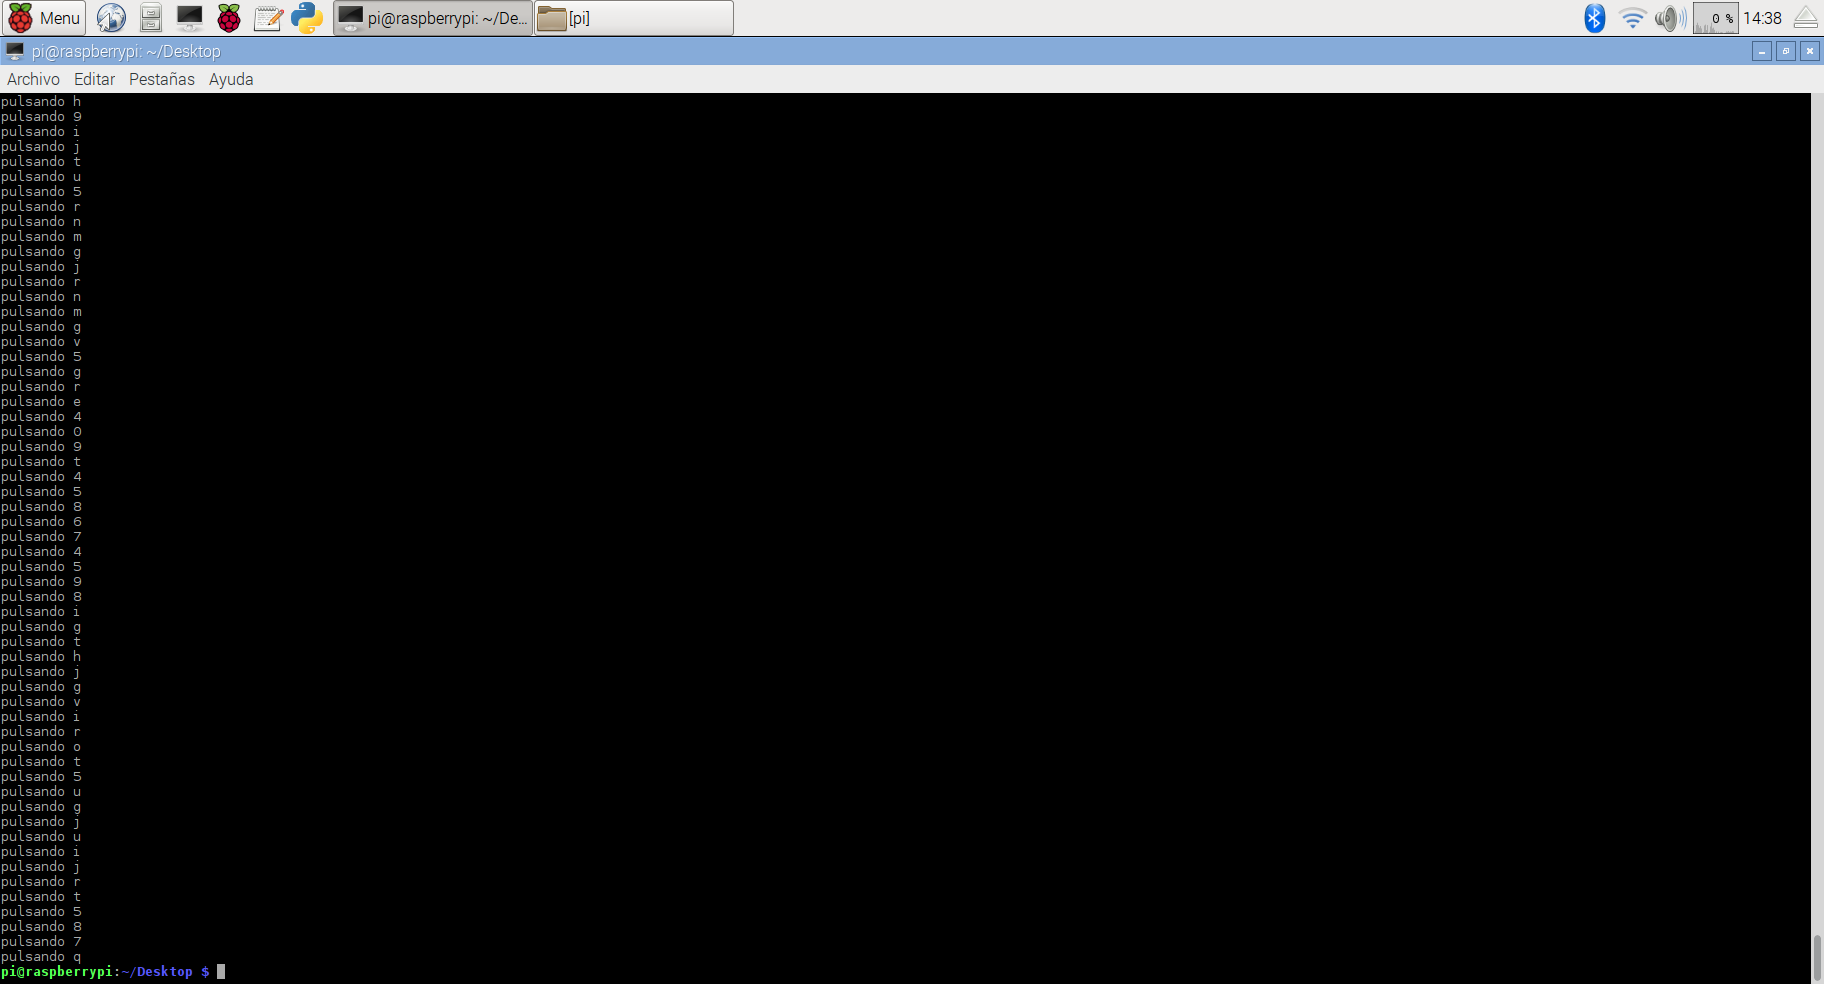
\includegraphics[scale = 0.25]{capitulo_04/figuras_dir/teclas.jpg}
    \caption{Eventos de pulsaciones de teclas}
    %\label{fig:figura4}
    \end{figure}

    \item Movimiento del ratón. Se incluyen las pulsaciones de los dos botones principales y deslizamientos de la ruleta central:\\
    
    \begin{itemize}
        \item Movimiento del ratón horizontalmente hacia la derecha:
        
            \begin{figure}
            \centering
            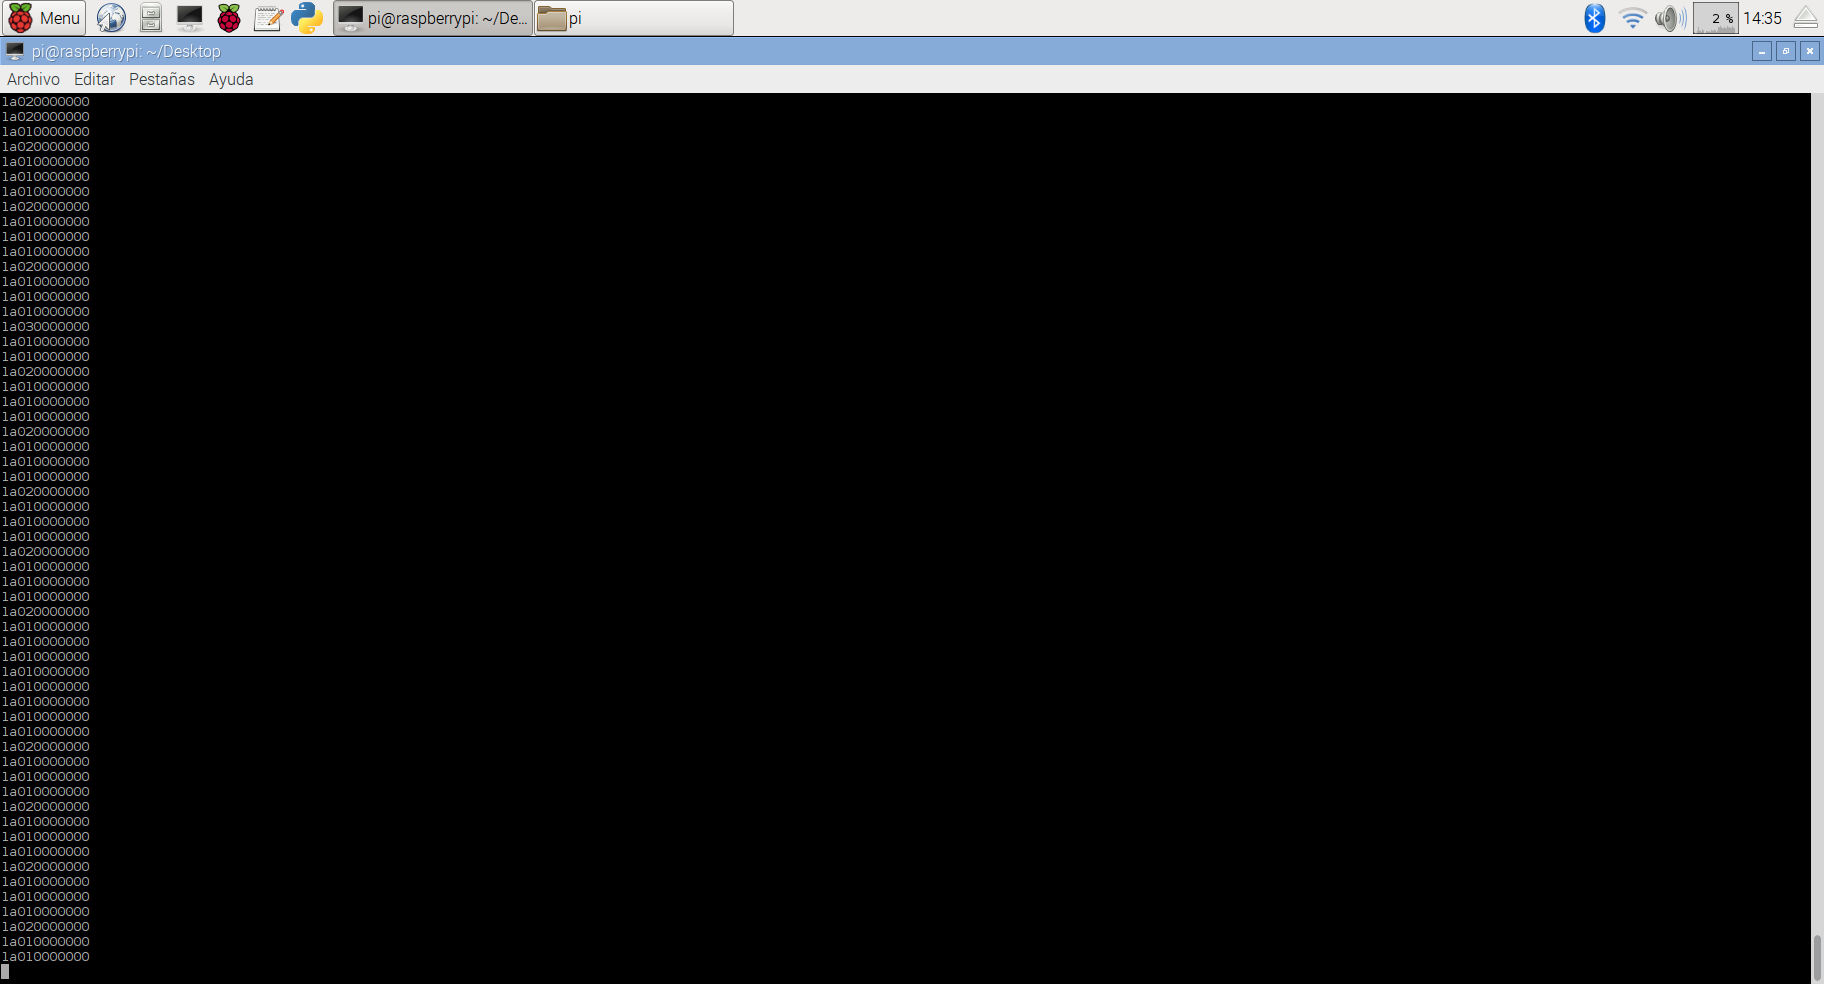
\includegraphics[scale = 0.25]{capitulo_04/figuras_dir/derecha.jpg}
            \caption{Eventos resultantes del movimiento del ratón horizontalmente hacia la derecha}
            %\label{fig:figura4}
            \end{figure}
        
        \item Movimiento del ratón horizontalmente hacia la izquierda:
        
            \begin{figure}
            \centering
            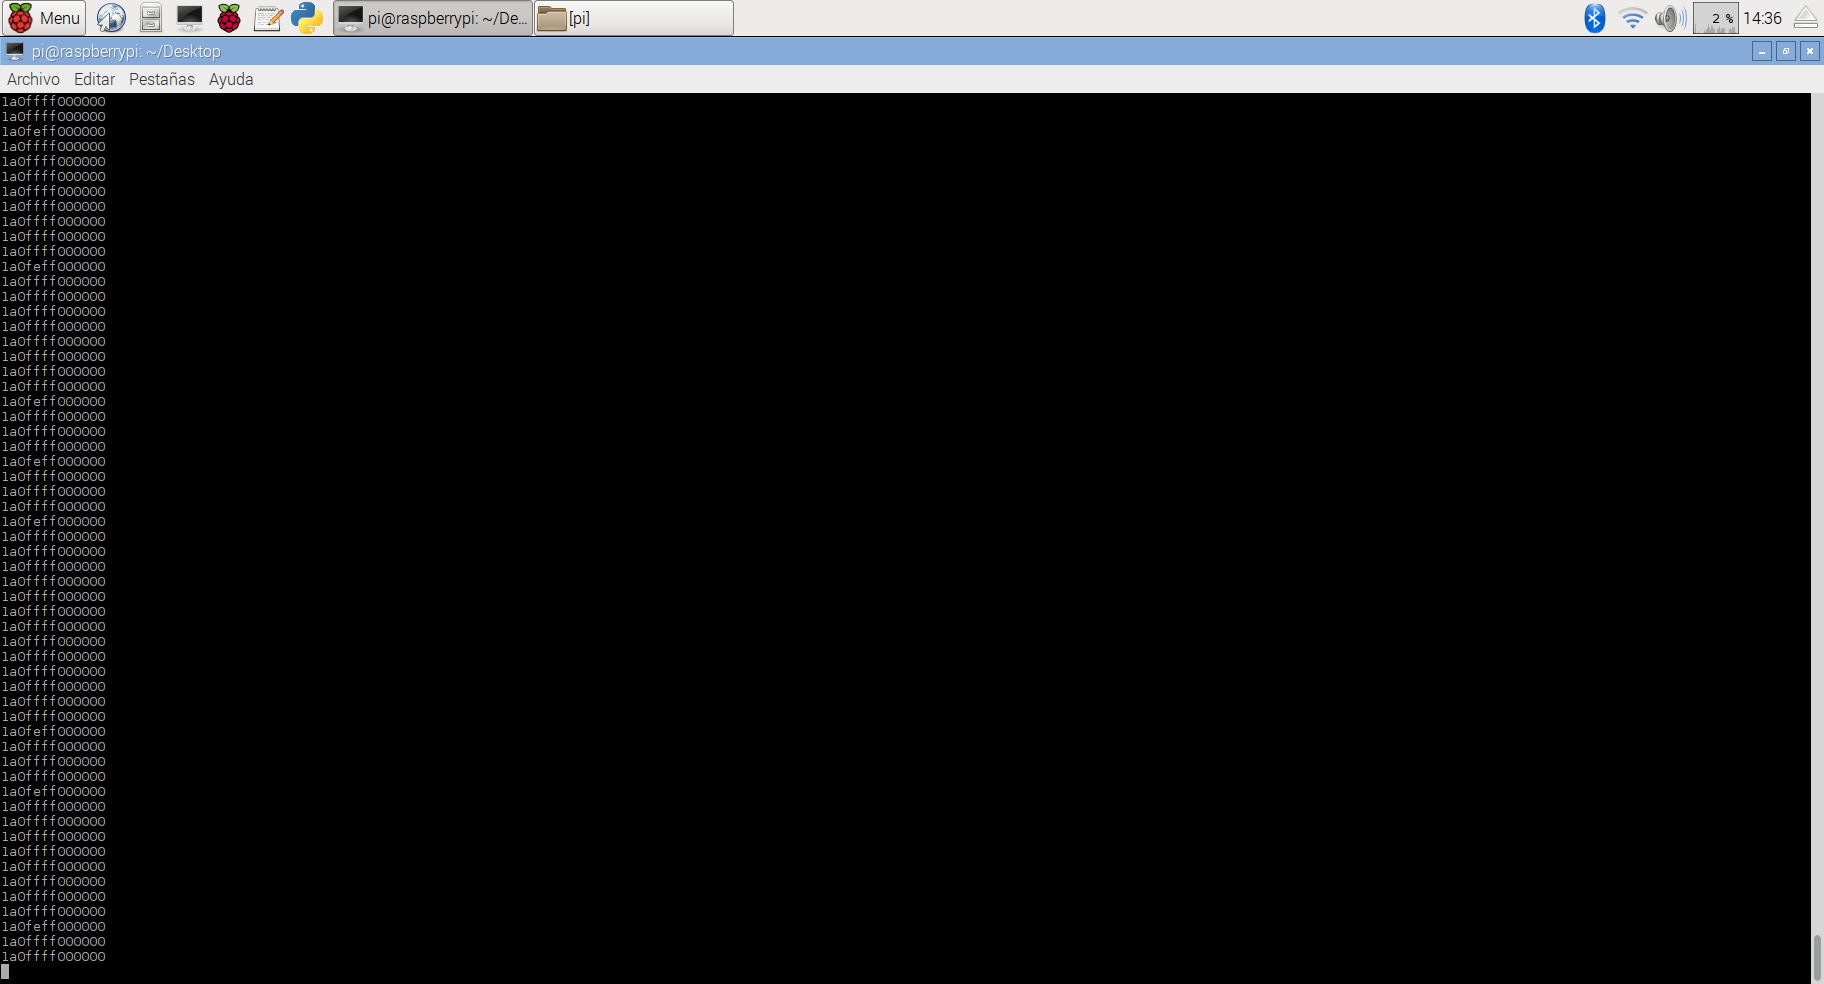
\includegraphics[scale = 0.25]{capitulo_04/figuras_dir/izquierda.jpg}
            \caption{Eventos resultantes del movimiento del ratón horizontalmente hacia la izquierda}
            %\label{fig:figura4}
            \end{figure}
        
        \item Movimiento del ratón verticalmente hacia arriba:
        
            \begin{figure}
            \centering
            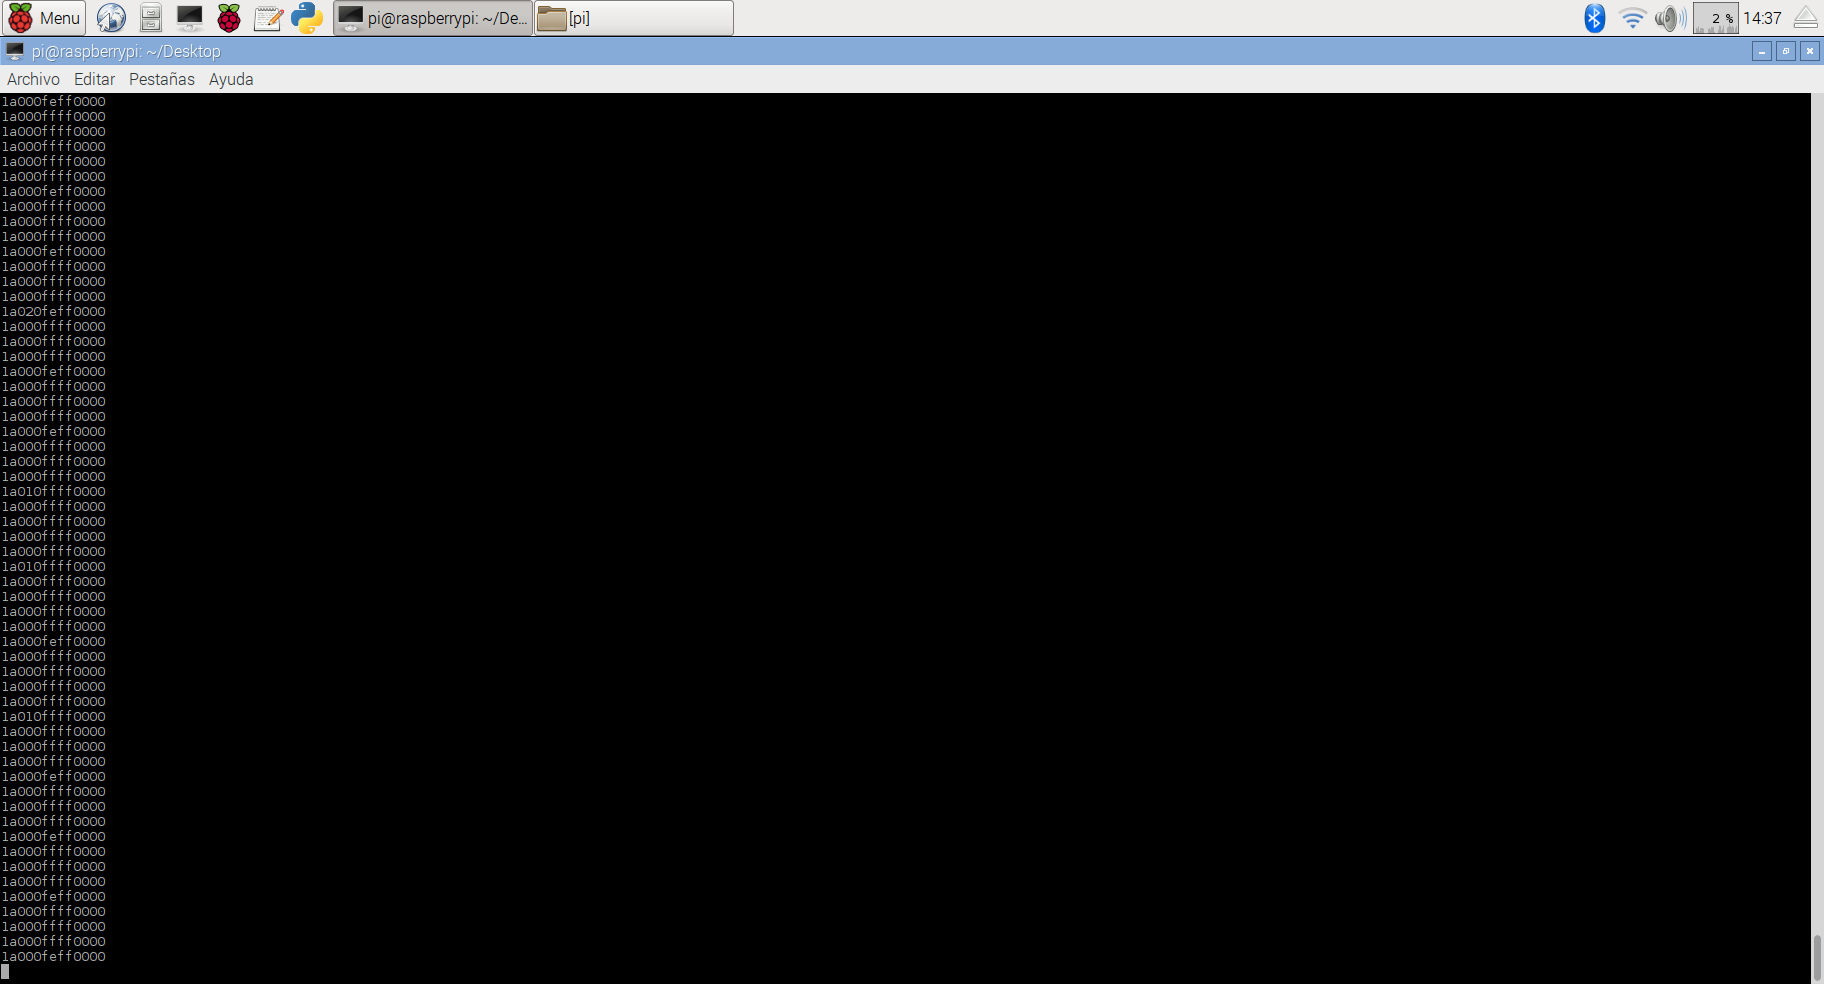
\includegraphics[scale = 0.25]{capitulo_04/figuras_dir/arriba.jpg}
            \caption{Eventos resultantes del movimiento del ratón verticalmente hacia arriba}
            %\label{fig:figura4}
            \end{figure}
        
        \item Movimiento del ratón verticalmente hacia abajo:
        
            \begin{figure}
            \centering
            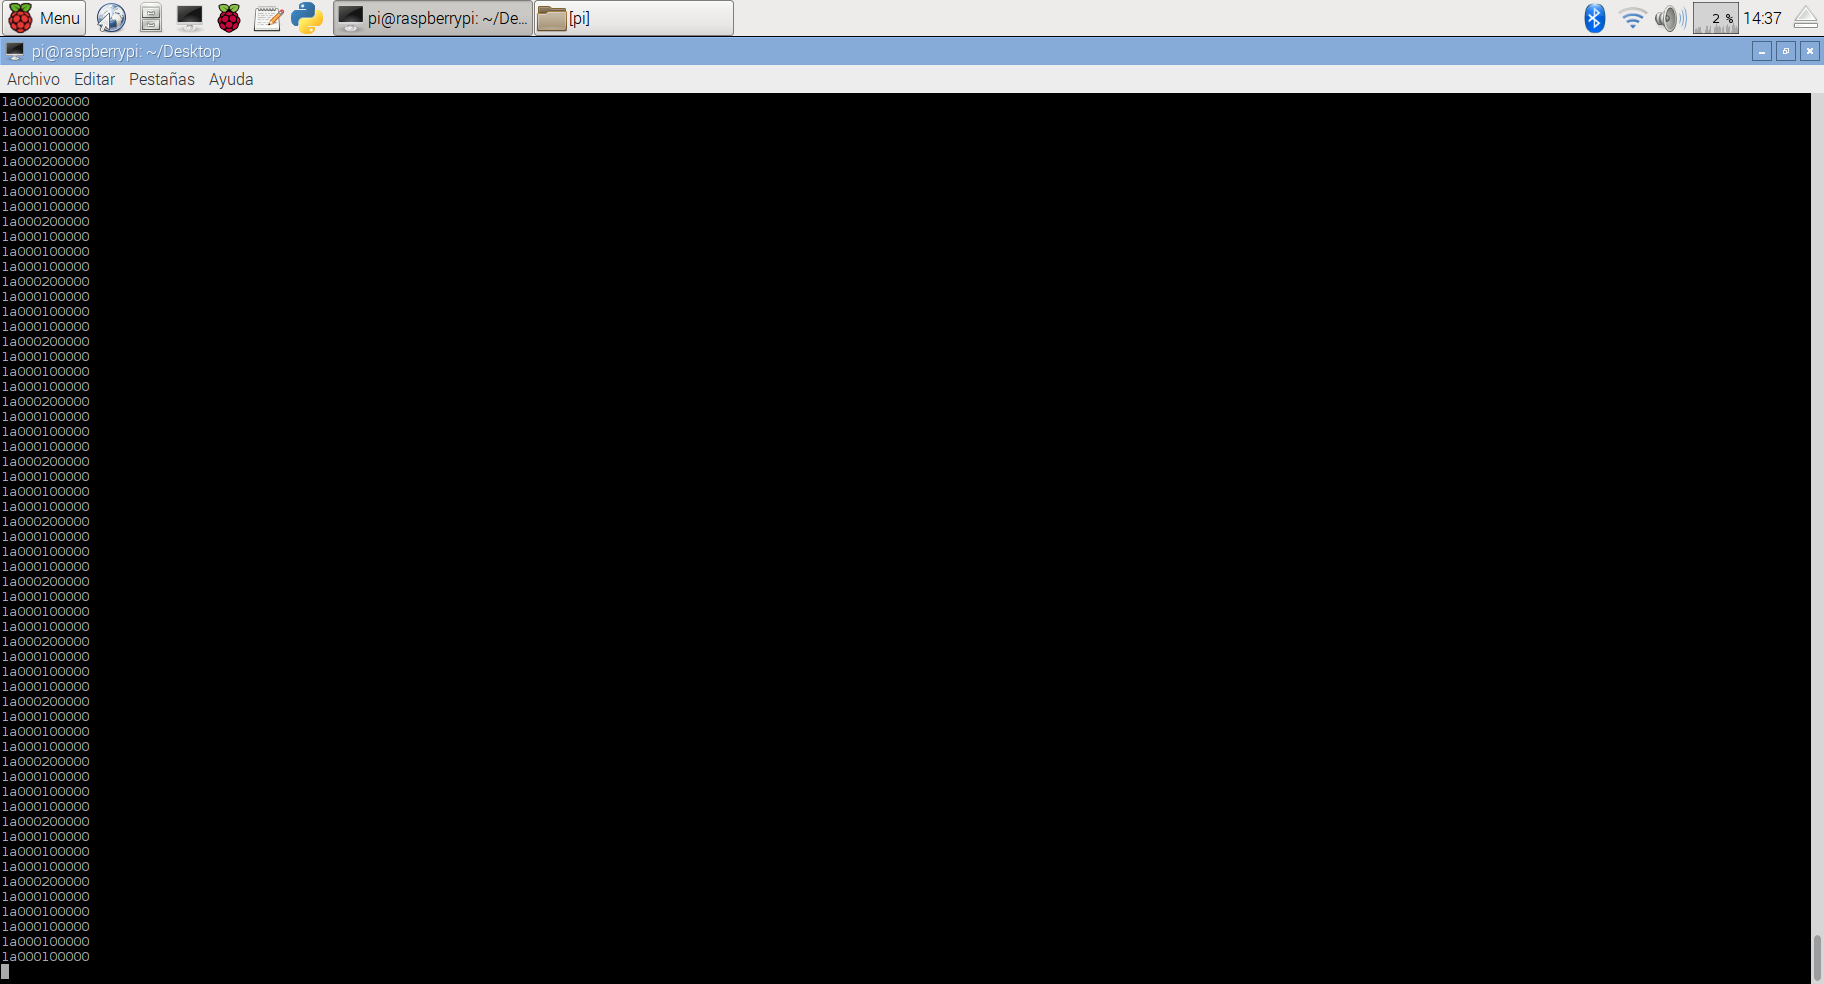
\includegraphics[scale = 0.25]{capitulo_04/figuras_dir/Abajo.jpg}
            \caption{Eventos resultantes del movimiento del ratón verticalmente hacia abajo}
            %\label{fig:figura4}
            \end{figure}
            
        \item Pulsaciones del botón derecho:
        
            \begin{figure}
            \centering
            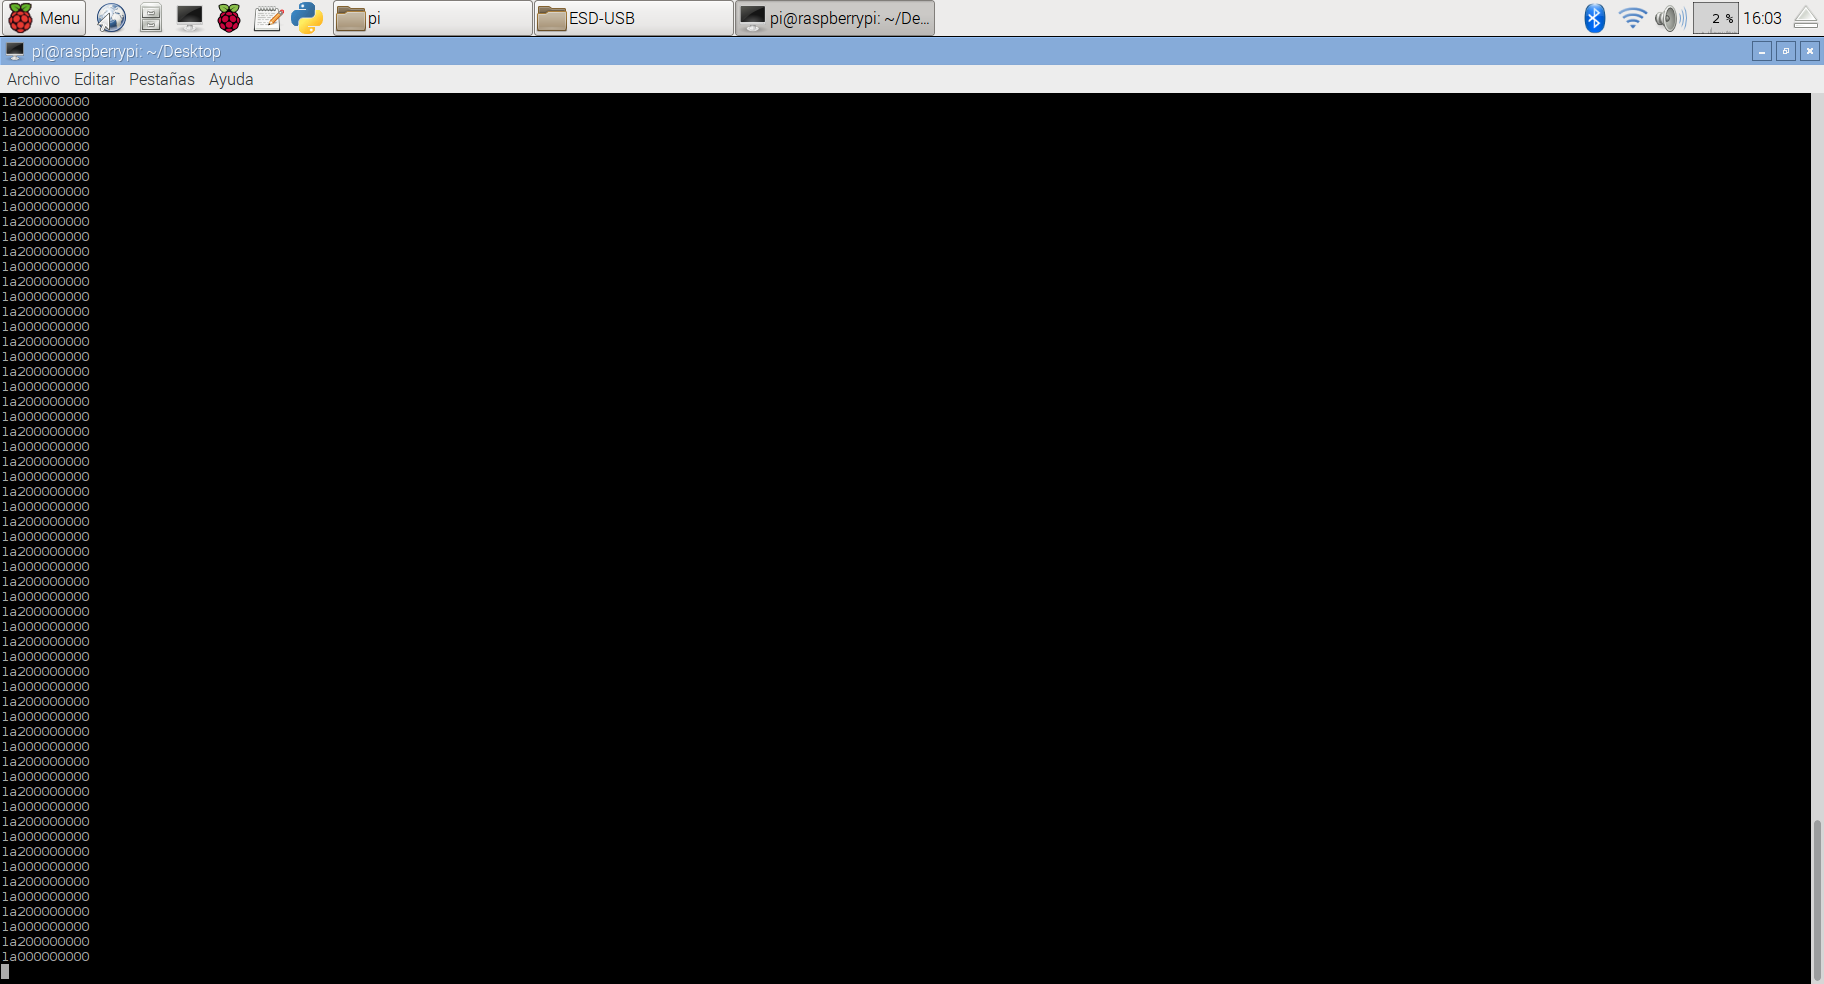
\includegraphics[scale = 0.25]{capitulo_04/figuras_dir/clickder.jpg}
            \caption{Eventos resultantes de las pulsaciones del botón derecho}
            %\label{fig:figura4}
            \end{figure}
        
        \item Pulsaciones del botón izquierdo:
        
            \begin{figure}
            \centering
            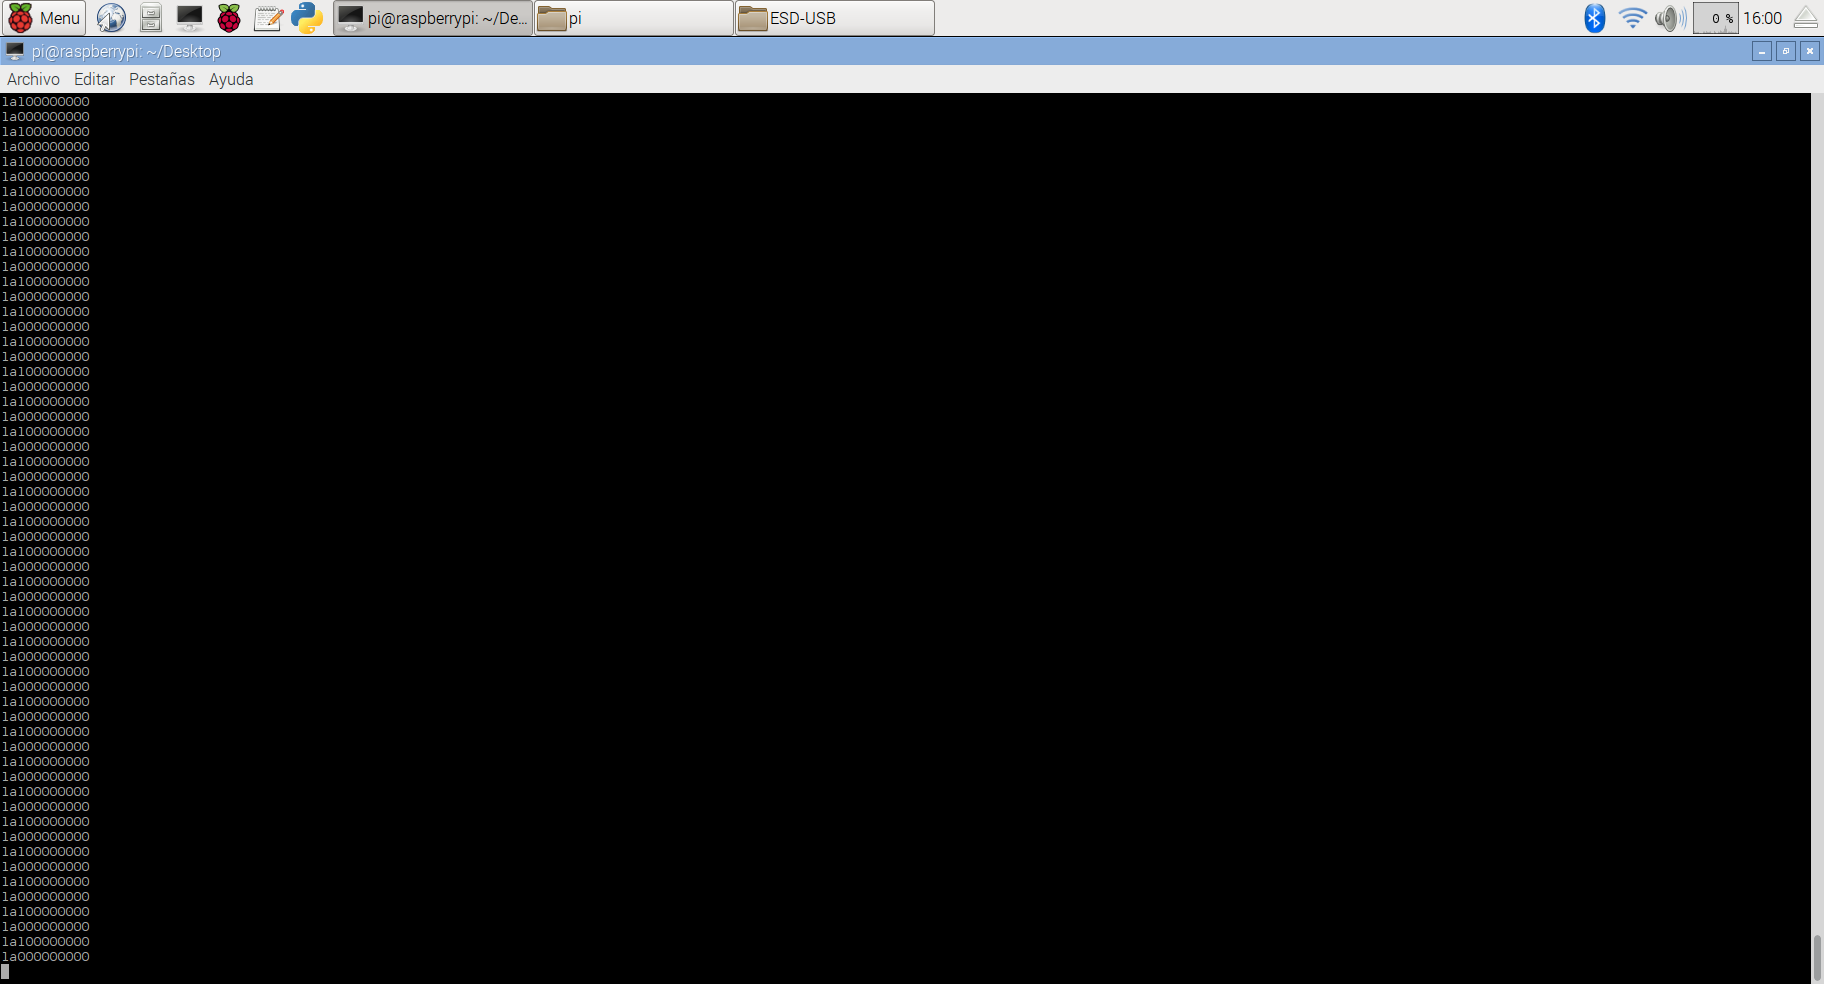
\includegraphics[scale = 0.25]{capitulo_04/figuras_dir/clickizq.jpg}
            \caption{Eventos resultantes de las pulsaciones del botón izquierdo}
            %\label{fig:figura4}
            \end{figure}
            
        \item Movimiento de la ruleta central hacia arriba:

            \begin{figure}
            \centering
            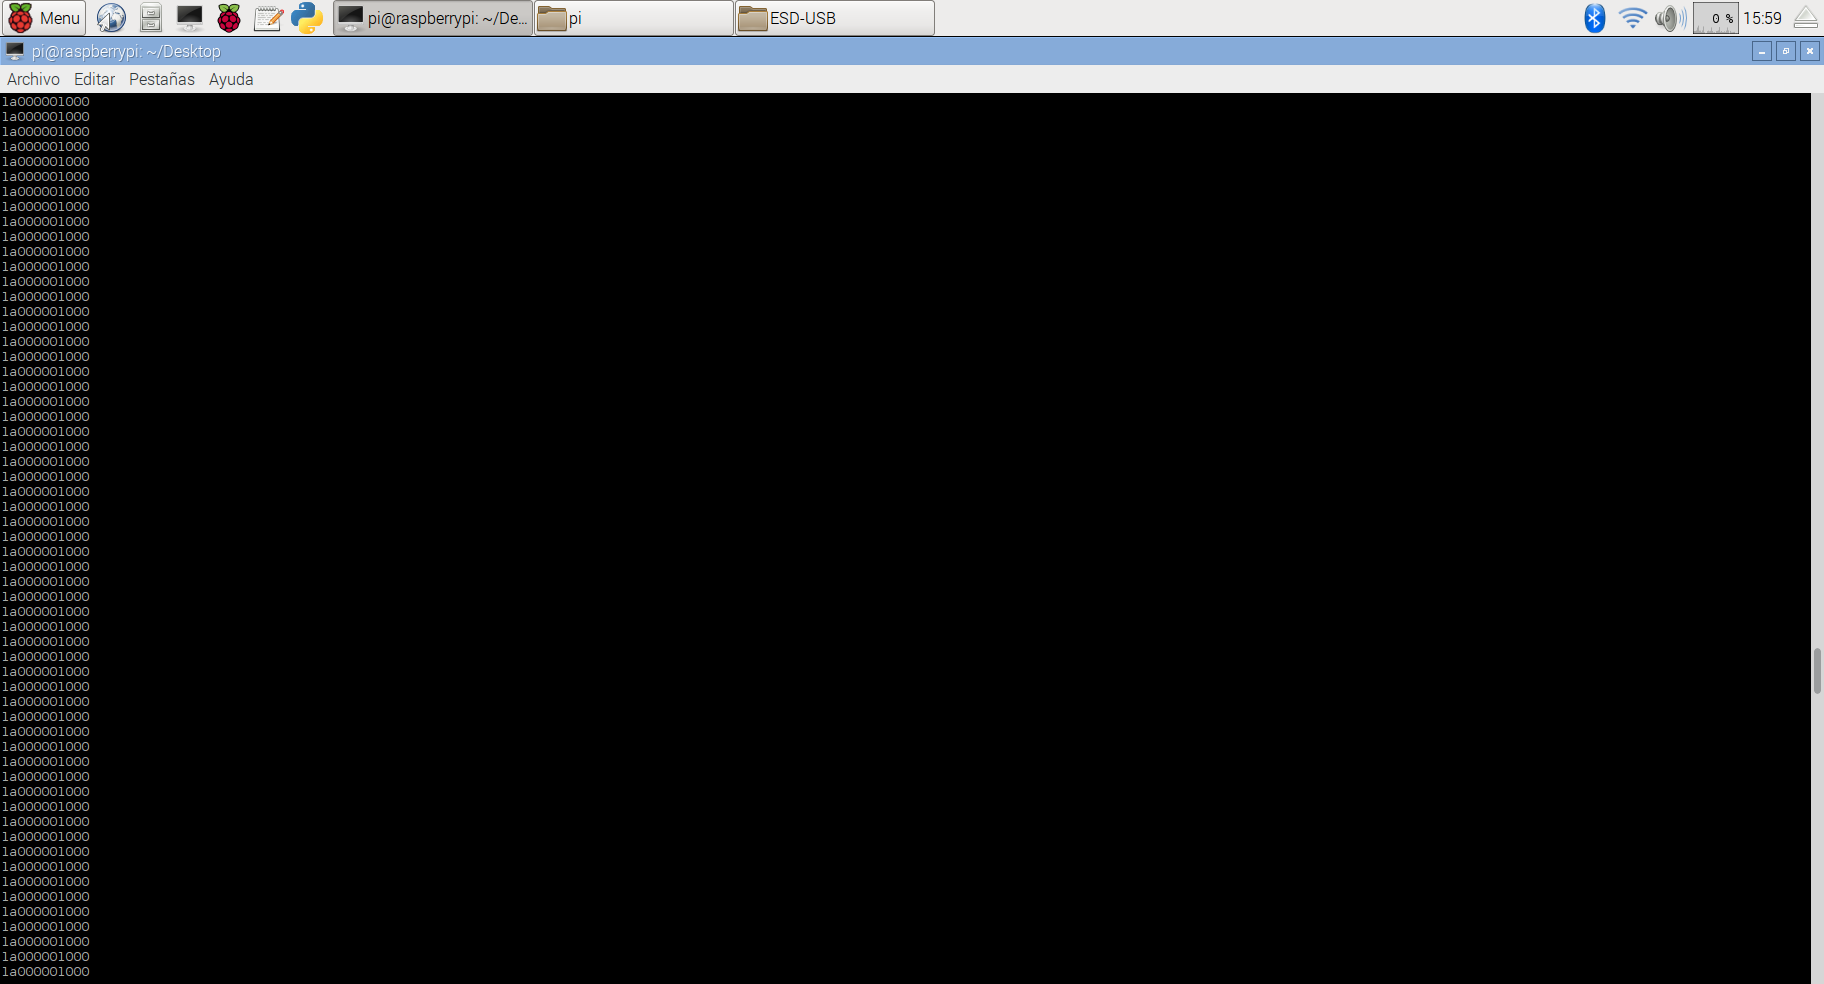
\includegraphics[scale = 0.25]{capitulo_04/figuras_dir/Raba.jpg}
            \caption{Eventos resultantes del movimiento de la ruleta hacia arriba}
            %\label{fig:figura4}
            \end{figure}
            
        \item Movimiento de la ruleta central hacia abajo:

            \begin{figure}
            \centering
            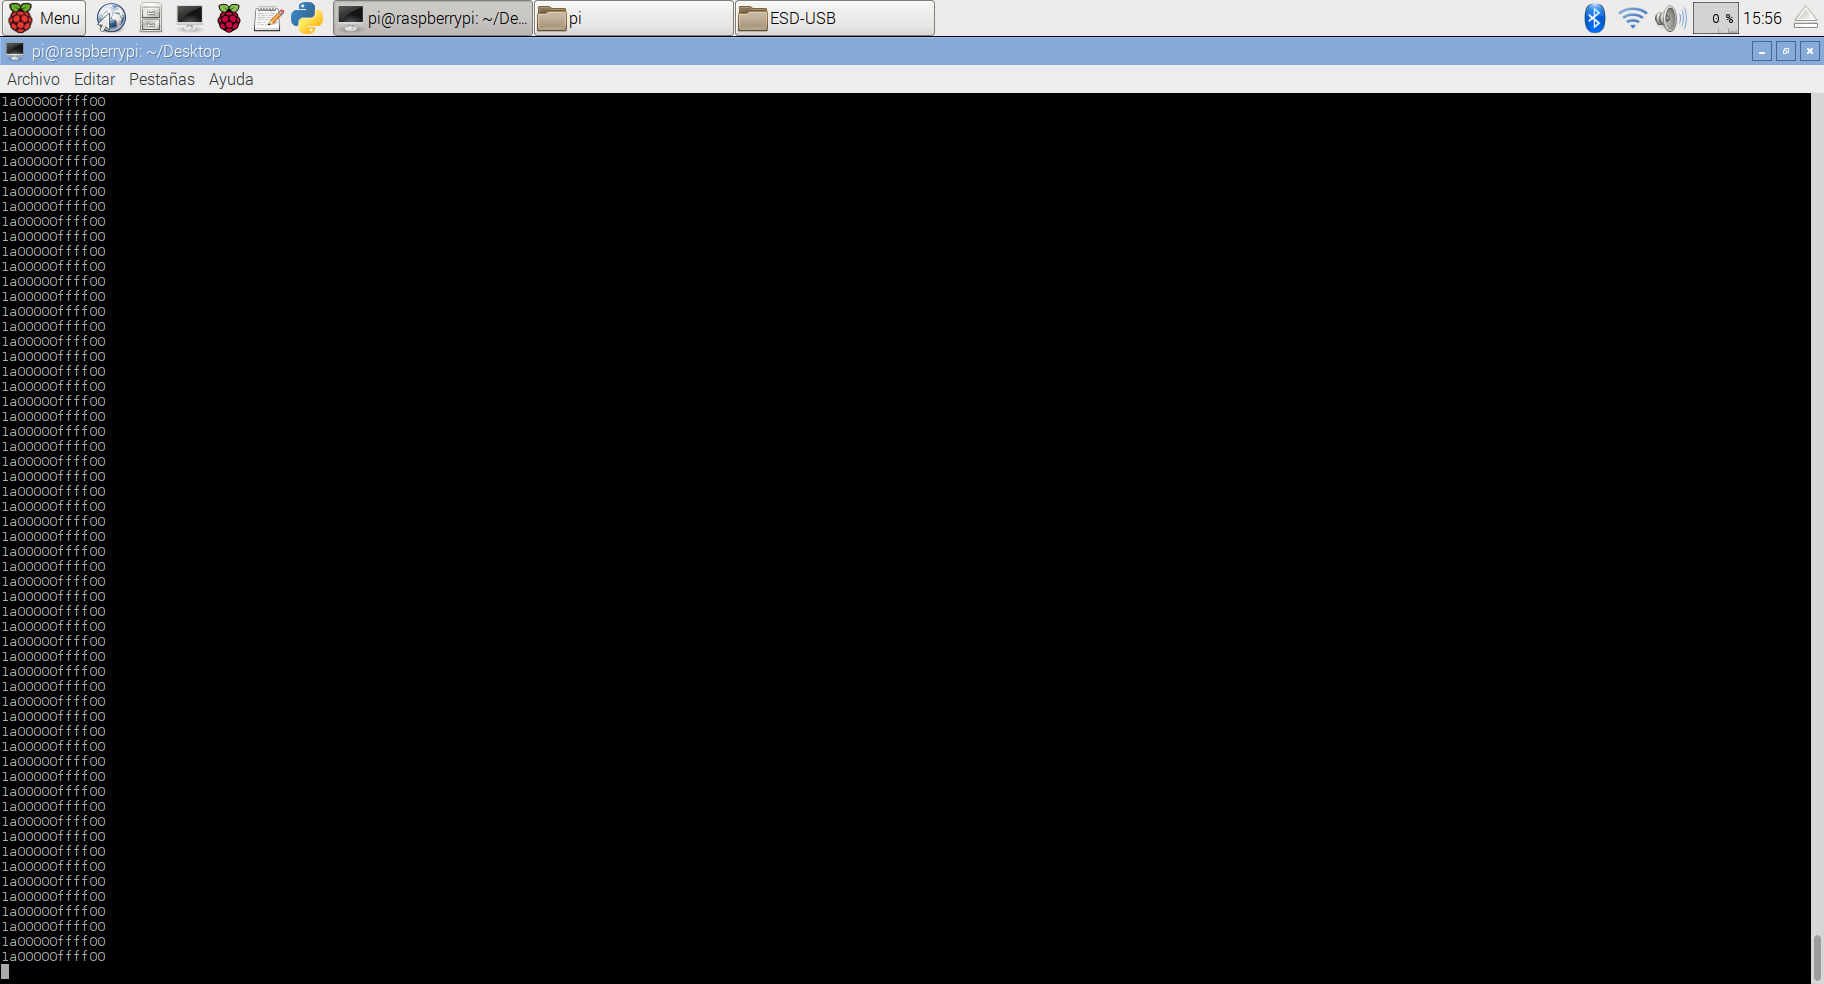
\includegraphics[scale = 0.25]{capitulo_04/figuras_dir/Rajo.jpg}
            \caption{Eventos resultantes del movimiento de la ruleta hacia abajo}
            %\label{fig:figura4}
            \end{figure}

    \end{itemize}

    
    \item Combinación de los eventos anteriores (demultiplexación):\\
\end{itemize}

    \begin{figure}
    \centering
    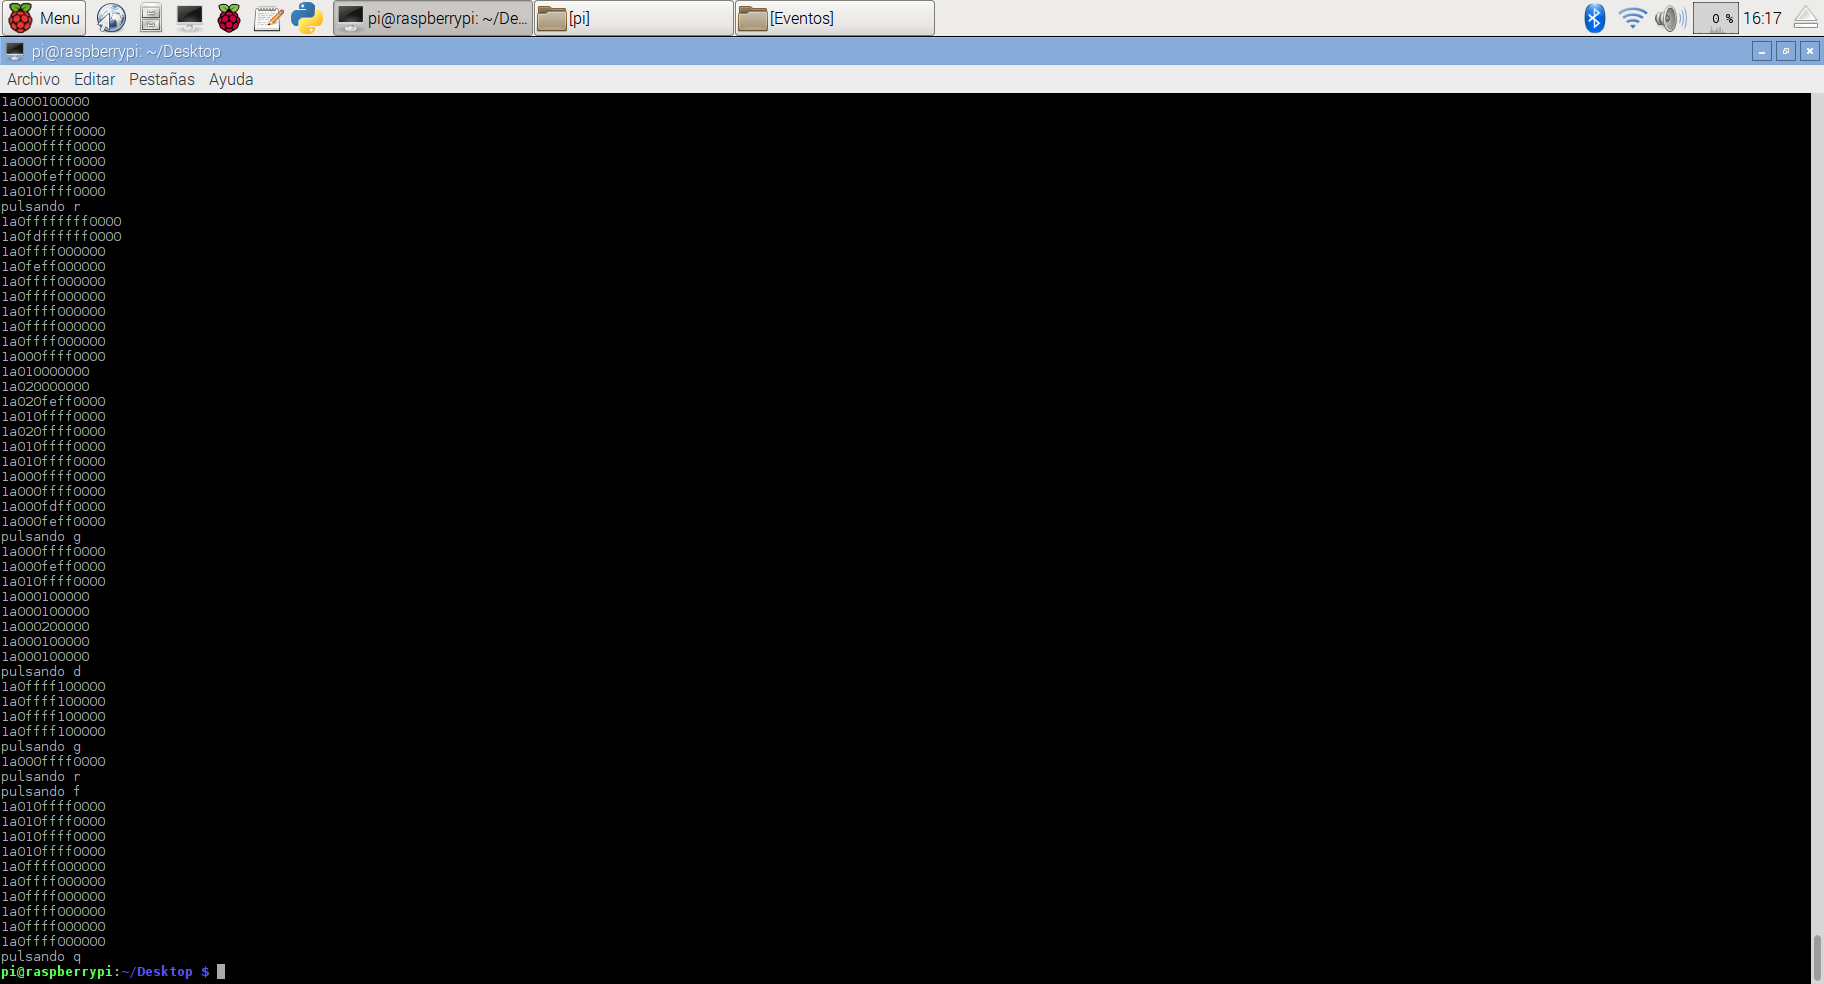
\includegraphics[scale = 0.25]{capitulo_04/figuras_dir/demu.jpg}
    \caption{Eventos demultiplexados}
    %\label{fig:figura4}
    \end{figure}


%%%%%%%%%%%%%%%%%%%%%%%%%%%%%%%%%%%%%%%%%%%%%%%%%%%%%%%
%		            	Seccion          			  %
%%%%%%%%%%%%%%%%%%%%%%%%%%%%%%%%%%%%%%%%%%%%%%%%%%%%%%%
\section{Proceso de calibración} \label{s4_2}

%%%%%%%%%%%%%%%%%%%%% Subsección %%%%%%%%%%%%%%%%%%%%%
\subsection{Instalación de ``OpenCV''} \label{s4_2_1}

Los pasos para realizar la instalación de OpenCV son:

\begin{enumerate}
    \item Instalación de las dependencias y compiladores:
    
\begin{bashcode}
$ sudo apt-get install build-
$ sudo apt-get install cmake git libgtk2.0-dev pkg-config \
    libavcodec-dev libavformat-dev libswscale-dev
$ sudo apt-get install python-dev python-numpy libtbb2 libtbb-dev \
    libjpeg-dev libpng-dev libtiff-dev libjasper-dev libdc1394-22-dev
\end{bashcode}
    
    \item Descargar OpenCV de la página oficial de OpenCV\citep{opencvorg}: ``https://opencv.org/releases.html''. Aparece una lista de versiones de esta biblioteca disponibles. En cualquiera de ellas se selecciona ``sources'' y automáticamente comienza la descarga en un archivo comprimido.
    
    \item Descomprimir el archivo y renombrarlo con un nombre mas sencillo para facilitar su manipulación como, por ejemplo ``OpenCV''.
    
    \item Crear una carpeta dentro de /OpenCV llamada ``build'':
    
\begin{bashcode}
$ cd OpenCV
$ mkdir build
$ cd build
\end{bashcode}
    
    \item Instalar el compilador ``cmake'':

\begin{bashcode}
$ cmake -D CMAKE_BUILD_TYPE=Release -D CMAKE_INSTALL_PREFIX=/usr/local ..
\end{bashcode}

    \item Ejecutar la orden ``make'' dentro de ``build'' para compilar toda la biblioteca:
\begin{bashcode}
$ make
\end{bashcode}

    \item Ejecutar la orden ``sudo make install'' para instalar la bilioteca:
\begin{bashcode}
$ sudo make install
\end{bashcode}

\end{enumerate}

%%%%%%%%%%%%%%%%%%%%% Subsección %%%%%%%%%%%%%%%%%%%%%
\subsection{Activación de la cámara} \label{s4_2_2}

Cuando se conecta el módulo de la cámara al puerto Cam por primera vez, lo más probable es que no esté activada. Para activarla, hay que acceder al menú de la configuración de Raspberry Pi a través del terminal:

\begin{bashcode}
$ sudo raspi-config
\end{bashcode}

A continuación, aparece el menú que presenta una amplia lista de elementos a configurar. La opción ``Interfacing Options'' permite acceder a la configuración de los periféricos. 

    \begin{figure}
    \centering
    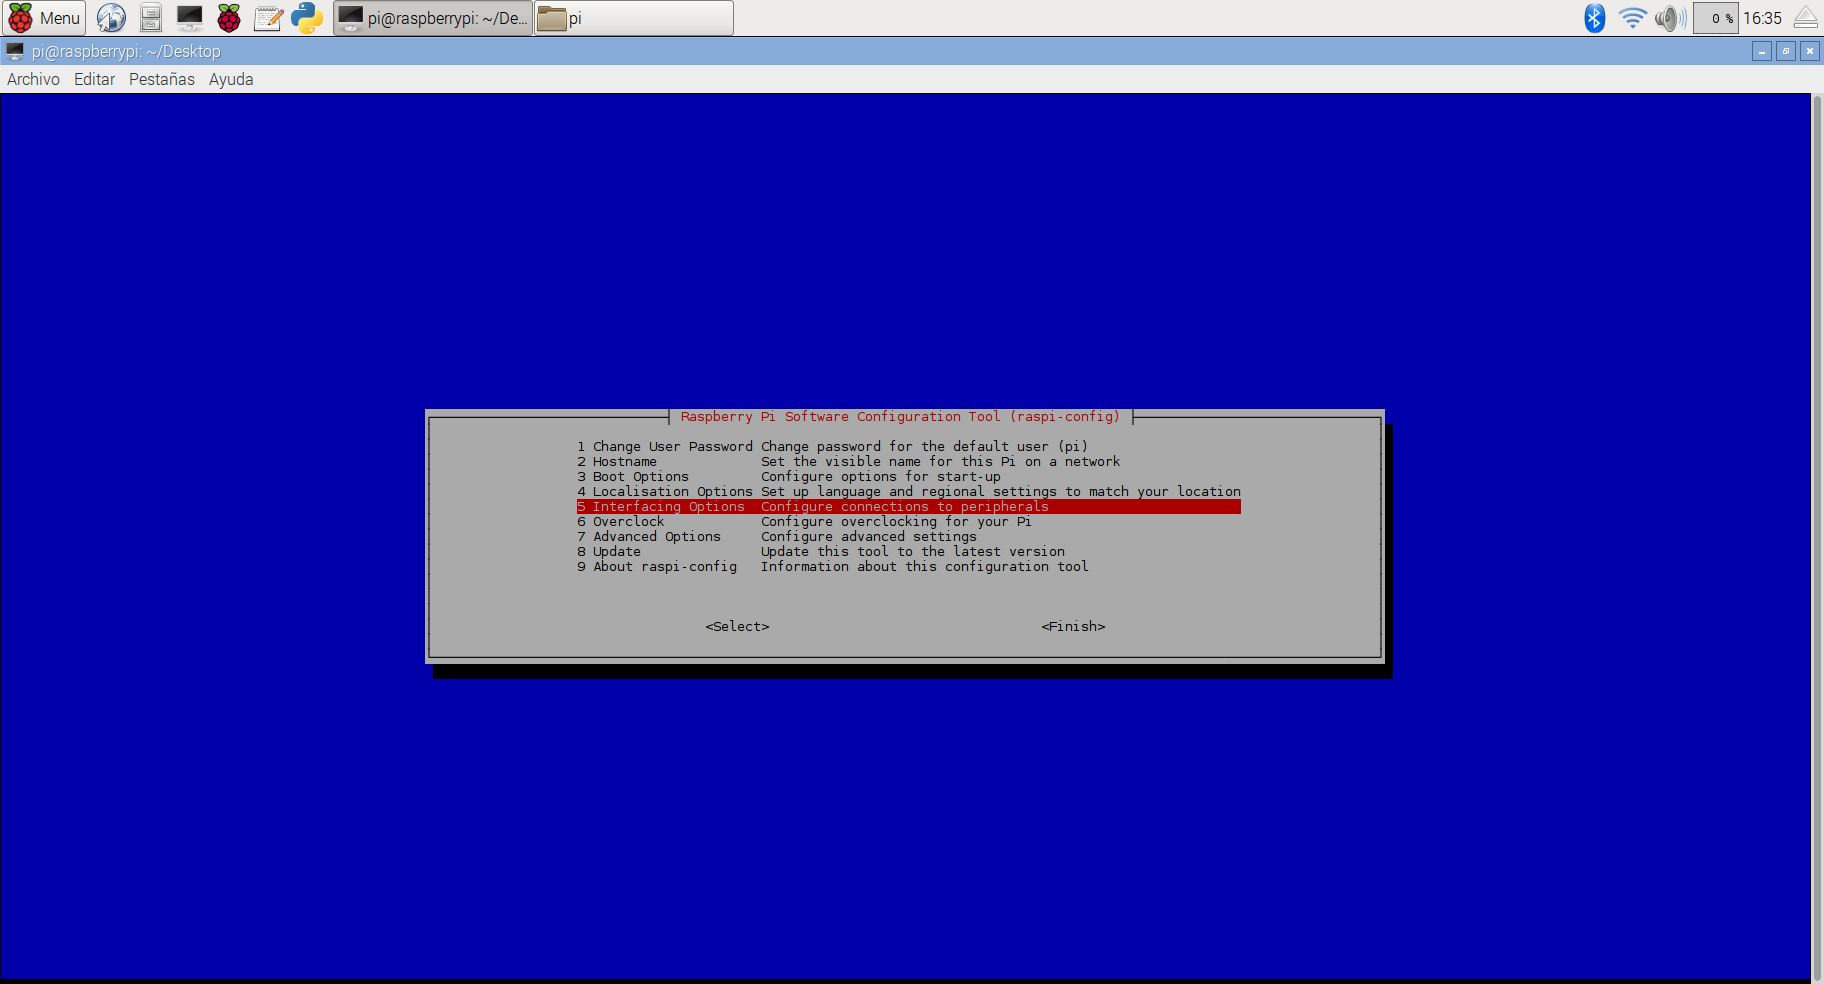
\includegraphics[scale = 0.25]{capitulo_04/figuras_dir/actp1.jpg}
    \caption{Menú de configuración}
    %\label{fig:figura4}
    \end{figure}

En este caso, interesa modificar el estado de ``camera’’ de ``disable’’ a ``enable’’. Posteriormente, se muestra el mensaje ``Would you like the camera interface to be enabled?’’ al cual hay que responder con ``$\lessdot$Enable$\gtrdot$’’ y reiniciar la microcontroladora para guardar y establecer los cambios correctamente. Esto va a permitir que ``eye\_detect.cpp’’ y ``save\_capture.cpp'' pueda encenderla para iniciar el proceso de detección y captura de imágenes.

    \begin{figure}
    \centering
    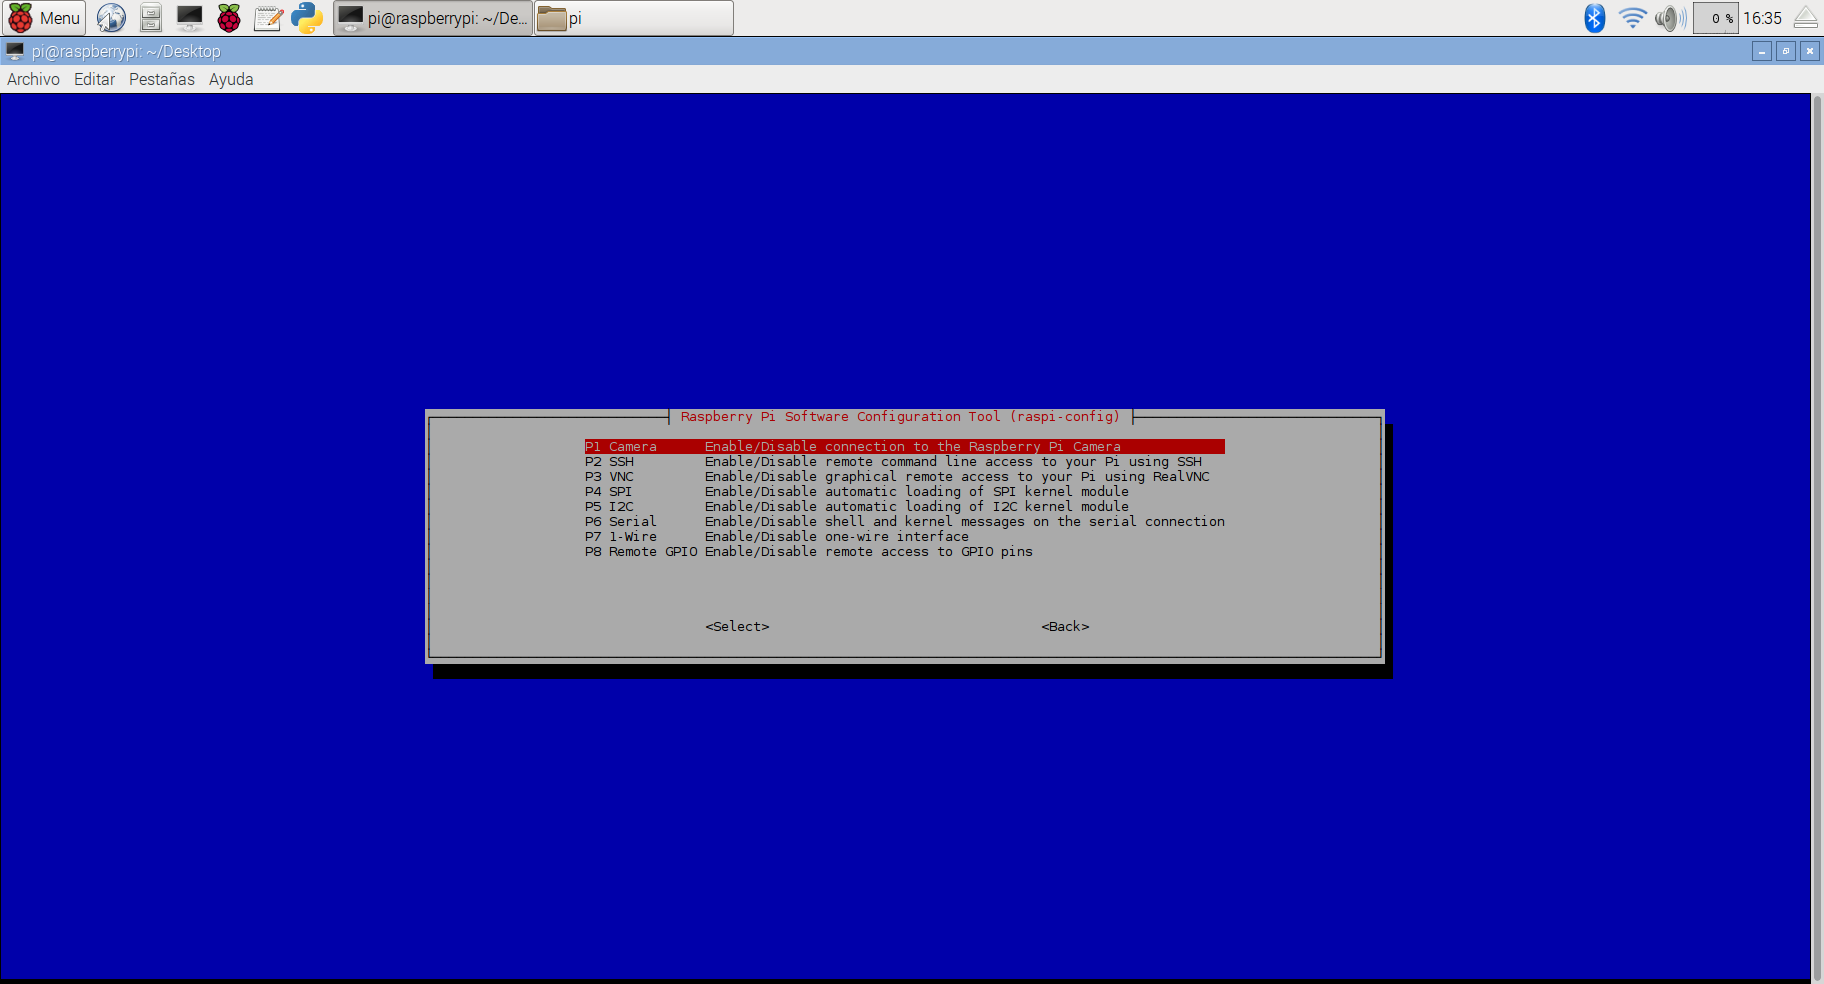
\includegraphics[scale = 0.25]{capitulo_04/figuras_dir/actp2.jpg}
    \caption{Submenú de ``Interfacing Options}
    %\label{fig:figura4}
    \end{figure}

    \begin{figure}
    \centering
    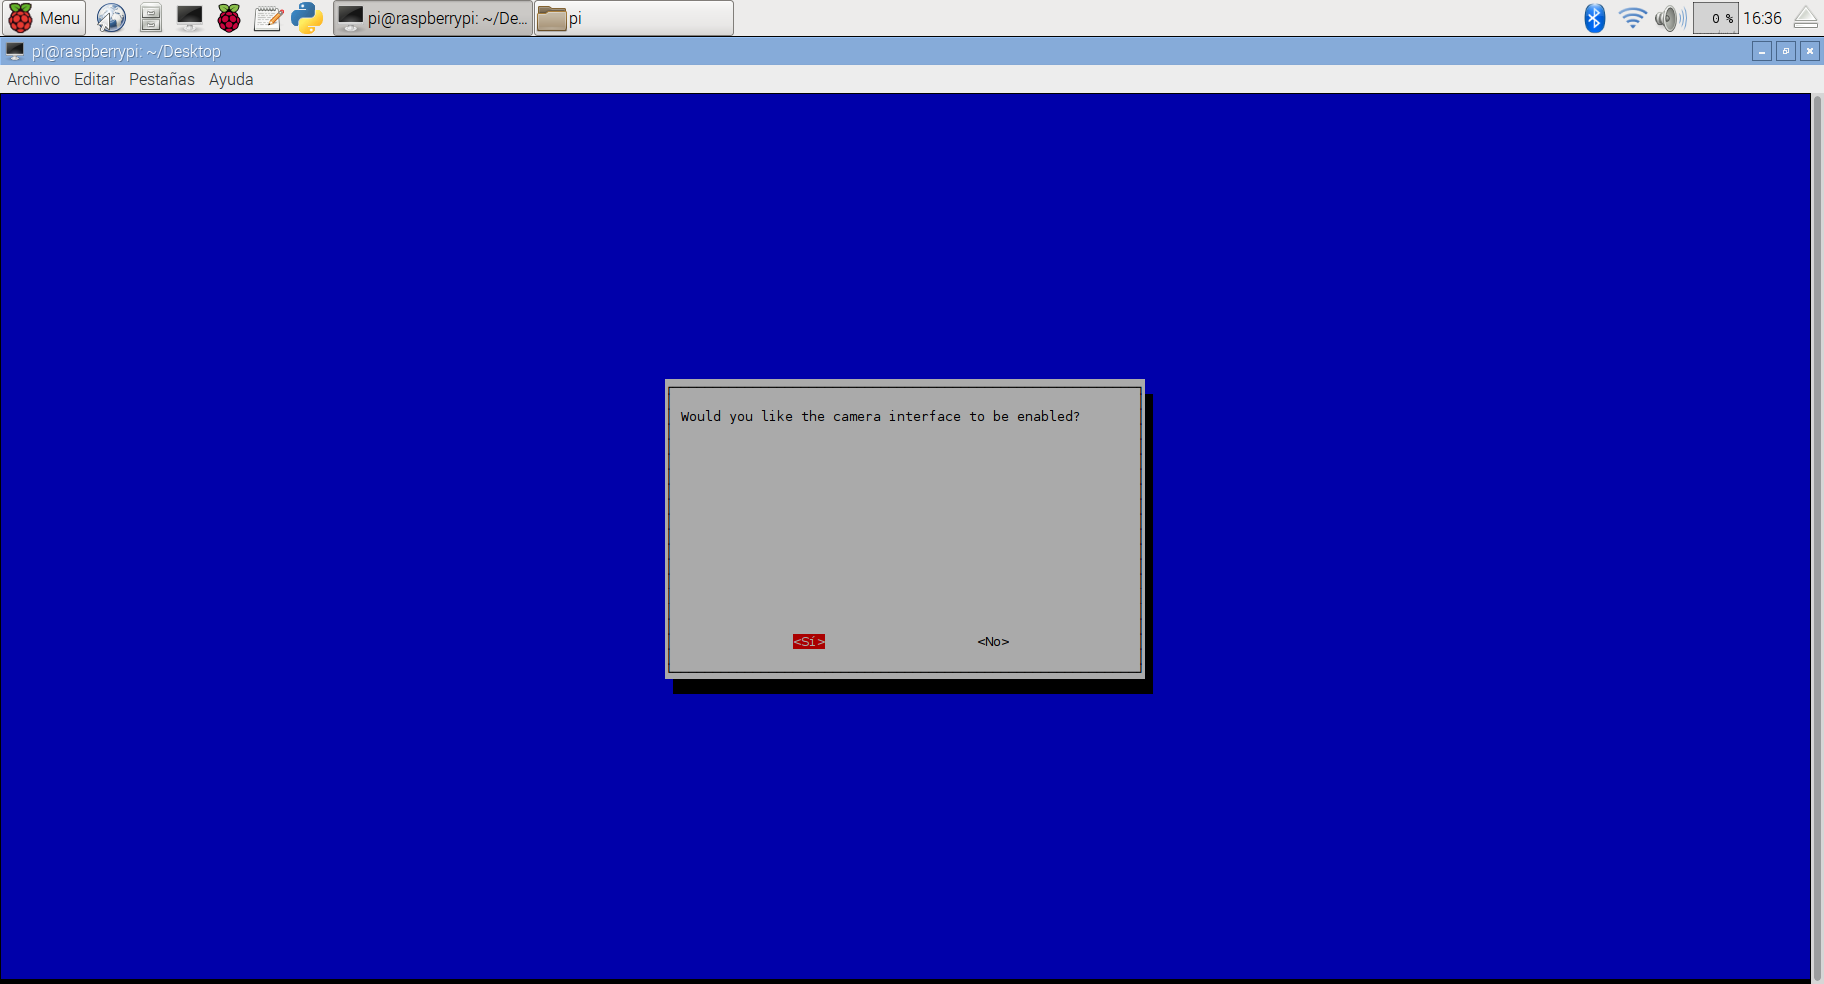
\includegraphics[scale = 0.25]{capitulo_04/figuras_dir/actp3.jpg}
    \caption{Mensaje de activación de la cámara}
    %\label{fig:figura4}
    \end{figure}


%%%%%%%%%%%%%%%%%%%%% Subsección %%%%%%%%%%%%%%%%%%%%%
\subsection{Resultados de la calibración} \label{s4_2_3}

Del proceso de calibración se obtienen dos tipos de resultados: las capturas tomadas con ayuda de ``save\_capture.cpp’’ y el archivo de calibración y los valores de los parámetros de la cámara obtenidos con ``catibration.cpp’’.

Al igual que en el caso anterior, es indispensable indicar las instrucciones de compilación al archivo ``makefile´´ para que conozca las direcciones de los archivos cabecera y archivos ``.c’’ así como los objetos de la biblioteca OpenCV invlolucrados en el proceso de creación del ejecutable tanto de ``save\_capture.cpp’’ como de ``calibration.cpp’’. Como ahora se trabaja con programas escritos en C++, el sistema Linux debe disponer del compilador ``g++’’. En caso de no tenerlo, se instala en el sistema tecleando los siguientes comandos en el terminal en el caso de Raspbian y de los sistemas operativos basados en Debian:

\begin{bashcode}
$ sudo apt-get install g++
\end{bashcode}

El siguiente paso consiste en redactar el contenido del ``makefile’’ o ``Makefile’’:

\begin{listing}
\begin{minted}[bgcolor=bg,
               frame=lines,
               framesep=2mm,
               linenos]
               {C}
save_capture: CXXFLAGS=`pkg-config --cflags opencv` --std=c++11
save_capture: LDLIBS=`pkg-config --libs opencv`
save_capture: CC=g++
save_capture: save_capture.o

calibration: CXXFLAGS=`pkg-config --cflags opencv` --std=c++11
calibration: LDLIBS=`pkg-config --libs opencv`
calibration: CC=g++
calibration: calibration.o

\end{minted}
\caption{Makefile de ``save\_capture.cpp'' y ``calibration.cpp''}
\label{Listing}
\end{listing}

Este archivo sirve para construir el ejecutable de ambos programas. Si ya se ha instalado OpenCV, se puede comenzar a construir los ejecutables y observar los resultados.

\begin{itemize}
    \item Capturas de imágenes:
    
    El archivo OpenCV se encuentra en la ruta ``Desktop/VKMS/Calibracion’’ junto al ``Makefile’’ anterior. \\
    
\begin{bashcode}
$ cd Desktop/VKMS/Calibracion
$ make save_capture
$ ./save_capture
\end{bashcode}
    
Después de ejecutar el programa, se abre una ventana que muestra todas las imágenes que captura la cámara y espera a que el usuario pulse alguna tecla. Cuando esto sucede, la imagen se captura y se guarda. Este proceso se lleva a cabo catorce veces. Como se ha comentado en apartados anteriores, cada captura corresponde con una posición concreta del patrón de calibración. Esto se puede observar en las imágenes capturadas y guardadas por el programa: \\
    
\begin{figure}[htbp]
\centering
\subfigure[Calibracion0.jpg]{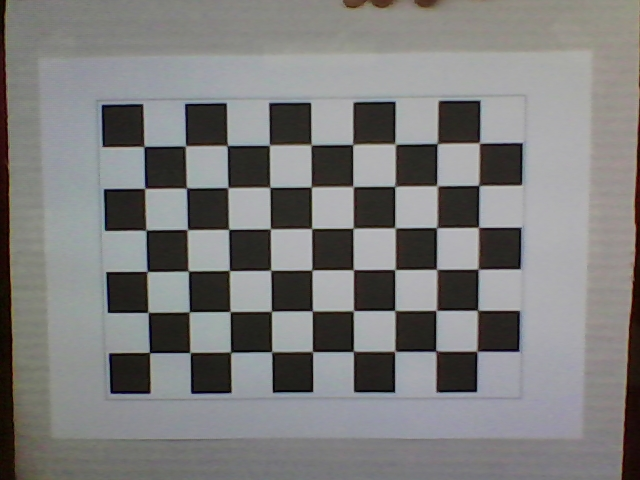
\includegraphics[width=50mm, scale = 0.3]{capitulo_04/figuras_dir/Calibracion0.jpg}}
\subfigure[Calibracion1.jpg]{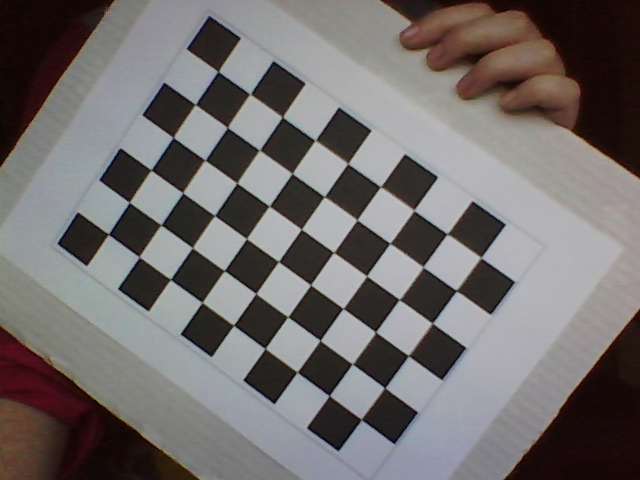
\includegraphics[width=50mm, scale = 0.3]{capitulo_04/figuras_dir/Calibracion1.jpg}}
\subfigure[Calibracion2.jpg]{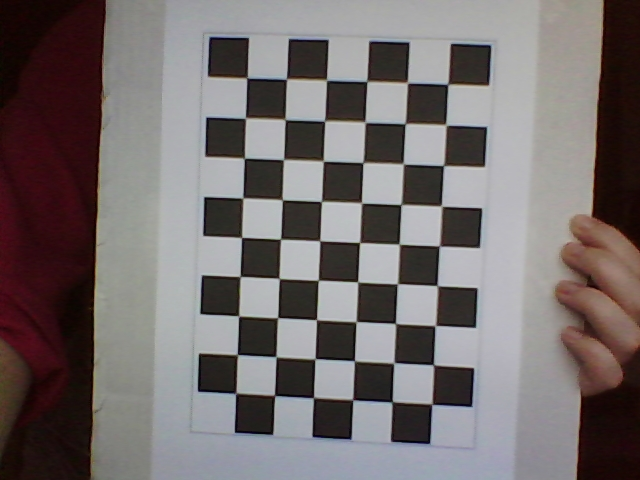
\includegraphics[width=50mm, scale = 0.3]{capitulo_04/figuras_dir/Calibracion2.jpg}}
\subfigure[Calibracion3.jpg]{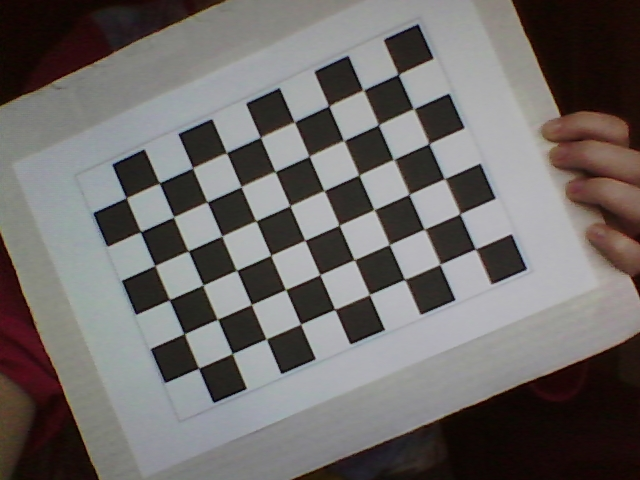
\includegraphics[width=50mm, scale = 0.3]{capitulo_04/figuras_dir/Calibracion3.jpg}}
\subfigure[Calibracion4.jpg]{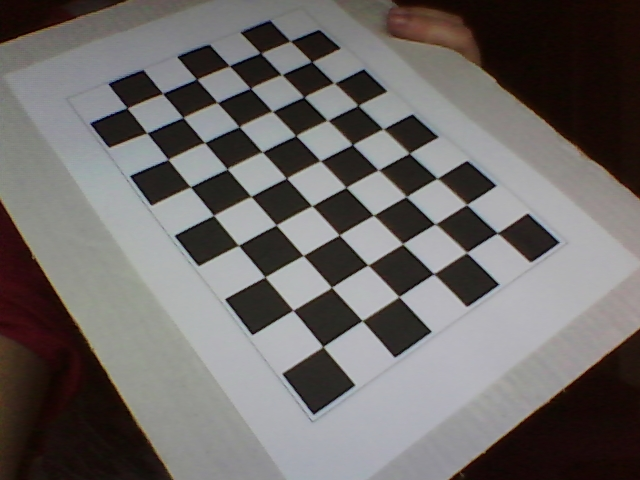
\includegraphics[width=50mm, scale = 0.3]{capitulo_04/figuras_dir/Calibracion4.jpg}}
\subfigure[Calibracion5.jpg]{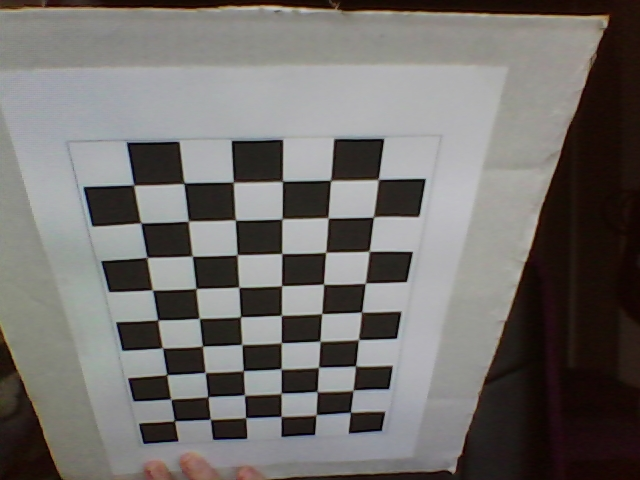
\includegraphics[width=50mm, scale = 0.3]{capitulo_04/figuras_dir/Calibracion5.jpg}}
\subfigure[Calibracion6.jpg]{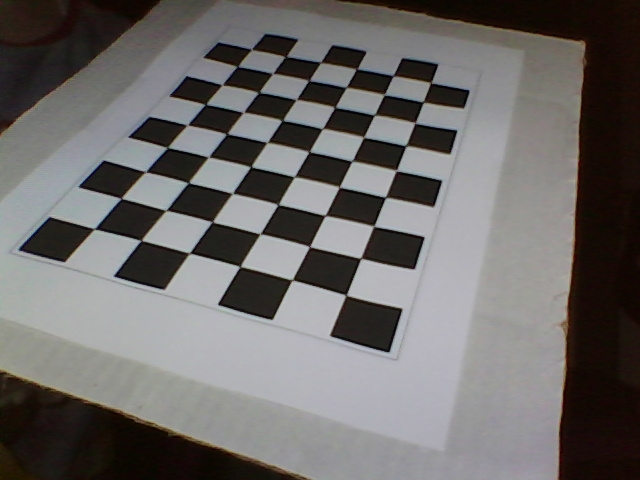
\includegraphics[width=50mm, scale = 0.3]{capitulo_04/figuras_dir/Calibracion6.jpg}}
\subfigure[Calibracion7.jpg]{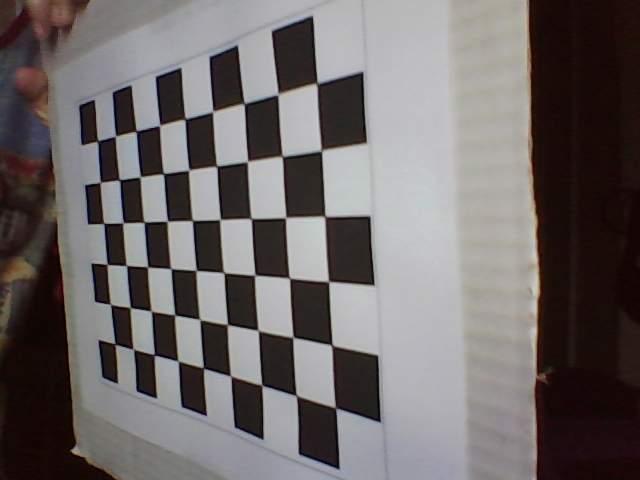
\includegraphics[width=50mm, scale = 0.3]{capitulo_04/figuras_dir/Calibracion7.jpg}}
\subfigure[Calibracion8.jpg]{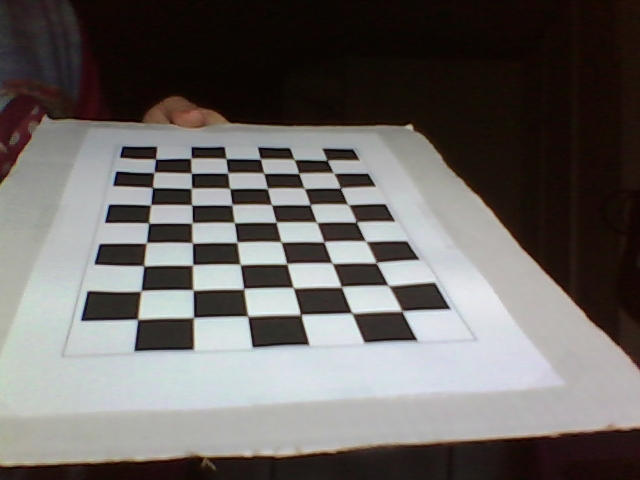
\includegraphics[width=50mm, scale = 0.3]{capitulo_04/figuras_dir/Calibracion8.jpg}}
\subfigure[Calibracion9.jpg]{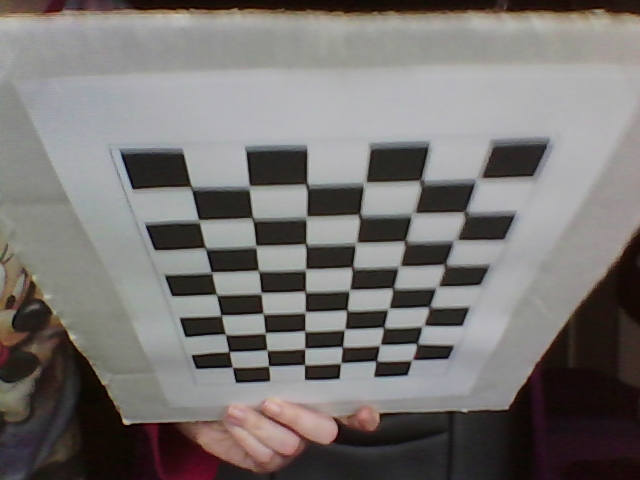
\includegraphics[width=50mm, scale = 0.3]{capitulo_04/figuras_dir/Calibracion9.jpg}}
\subfigure[Calibracion10.jpg]{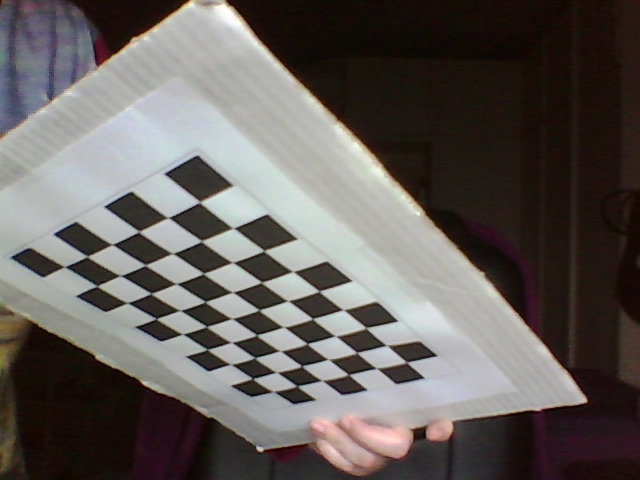
\includegraphics[width=50mm, scale = 0.3]{capitulo_04/figuras_dir/Calibracion10.jpg}}
\subfigure[Calibracion11.jpg]{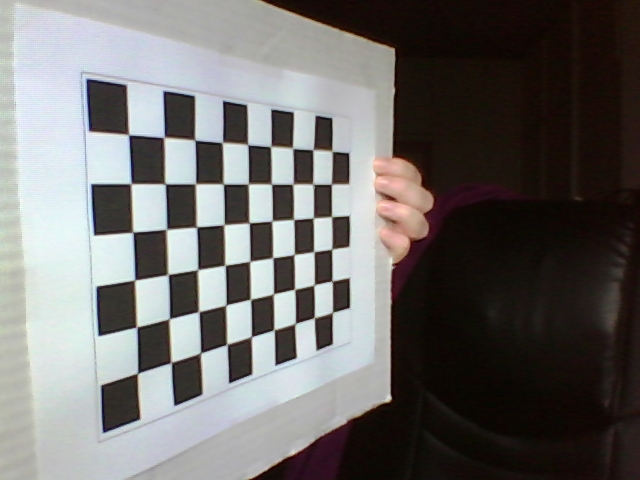
\includegraphics[width=50mm, scale = 0.3]{capitulo_04/figuras_dir/Calibracion11.jpg}}
\subfigure[Calibracion12.jpg]{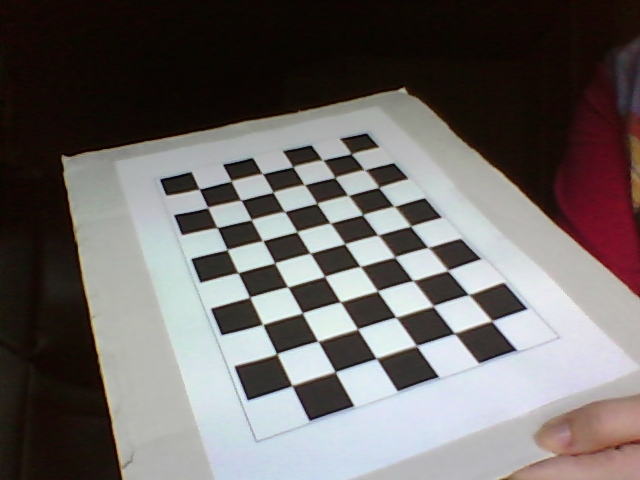
\includegraphics[width=50mm, scale = 0.3]{capitulo_04/figuras_dir/Calibracion12.jpg}}
\subfigure[Calibracion13.jpg]{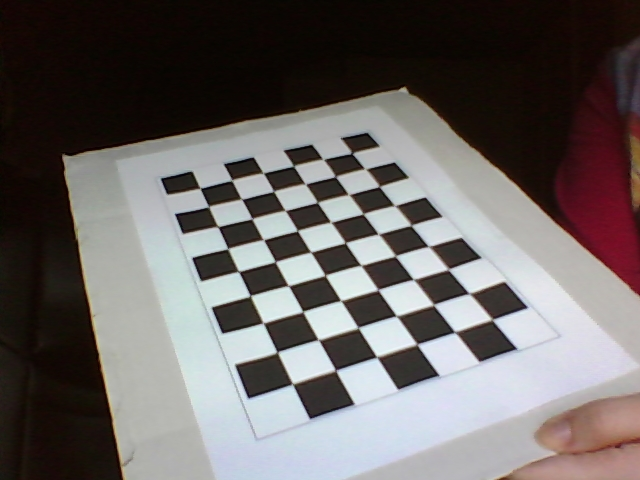
\includegraphics[width=50mm, scale = 0.3]{capitulo_04/figuras_dir/Calibracion13.jpg}}
\caption{Imágenes capturadas y guardadas por ``save\_capture.cpp''} 
%\label{fig:lego}
\end{figure}

    \item Calibración:

El ejecutable se obtiene y ejecuta de la misma forma que con ``save\_capture.cpp’’: \\

\begin{bashcode}
$ cd Desktop/VKMS/Calibracion
$ make calibration
$ ./calibration
\end{bashcode}

El programa lee las imágenes que fueron guardadas en el paso anterior, detecta el patrón en cada una, calcula los puntos de las esquinas interiores de los cuadrados, dibuja el patrón si lo ha detectado, obtiene los parámetros de la cámara, los representan en el terminal y finalmente, los introduce en ``MiCam.yml’’:

\begin{itemize}
    \item Representación visual de los patrones sobre las capturas:\\
    
\begin{figure}[htbp]
\centering
\subfigure[Posición 1]{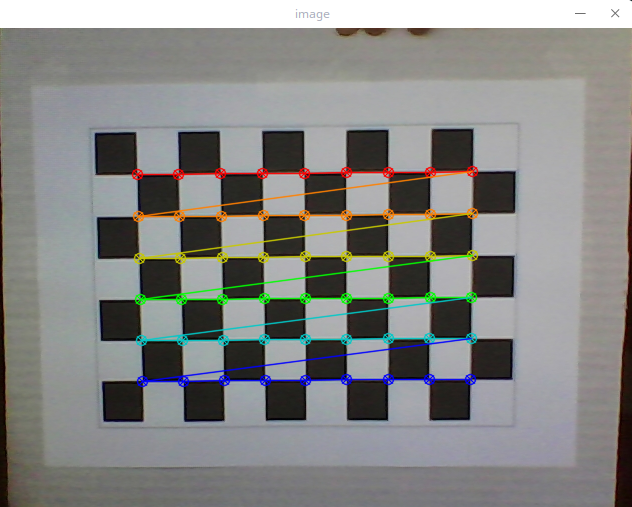
\includegraphics[width=50mm]{capitulo_04/figuras_dir/pat1.jpg}}
\subfigure[Posición 2]{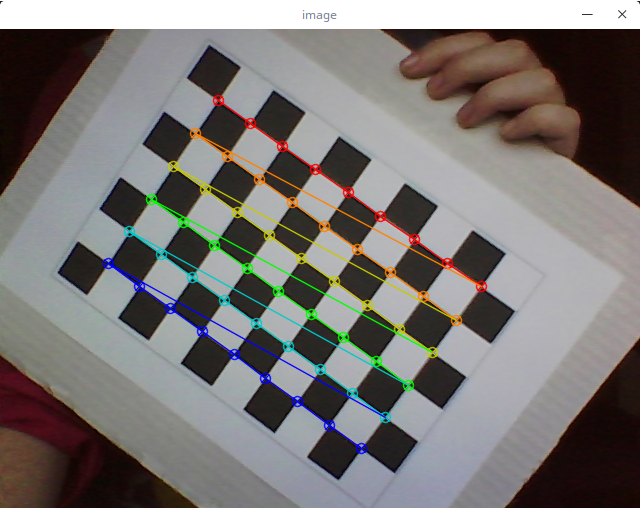
\includegraphics[width=50mm, scale = 0.3]{capitulo_04/figuras_dir/pat2.jpg}}
\subfigure[Posición 3]{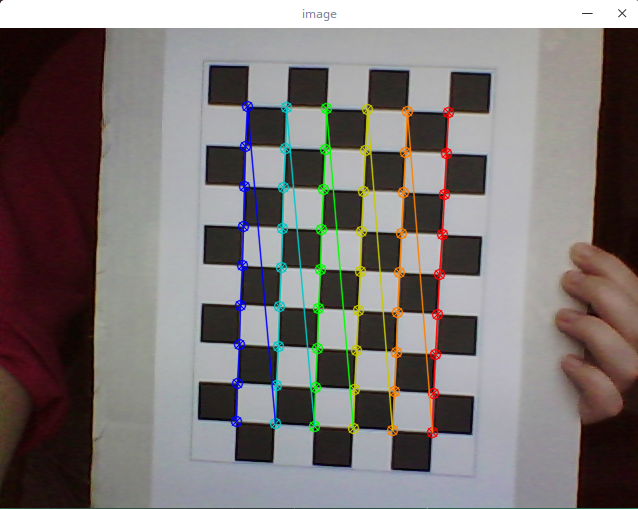
\includegraphics[width=50mm, scale = 0.3]{capitulo_04/figuras_dir/pat3.jpg}}
\subfigure[Posición 4]{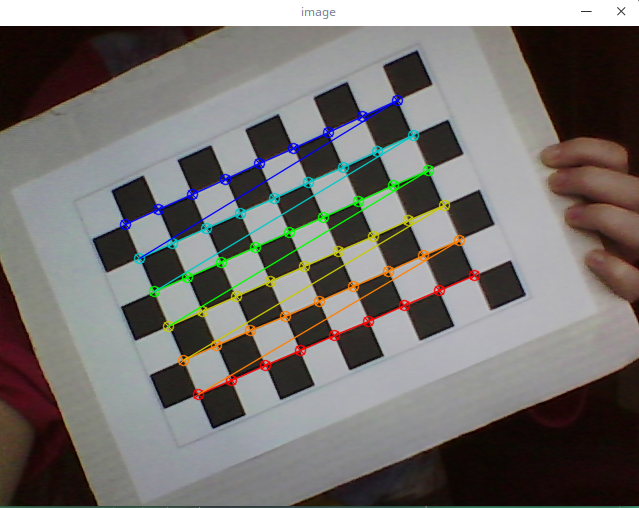
\includegraphics[width=50mm, scale = 0.3]{capitulo_04/figuras_dir/pat4.jpg}}
\subfigure[Posición 5]{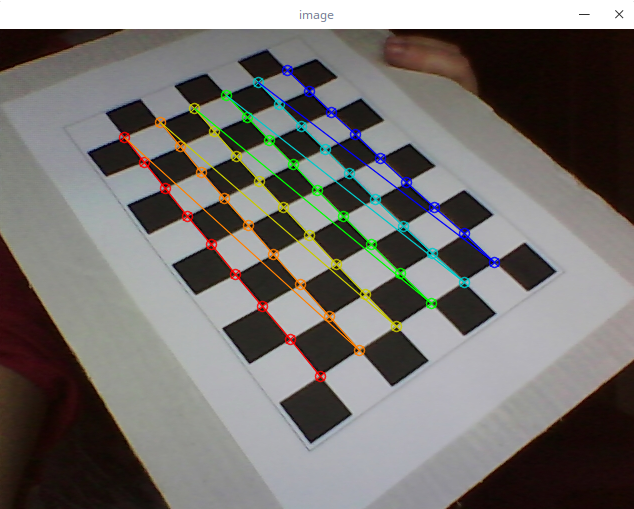
\includegraphics[width=50mm, scale = 0.3]{capitulo_04/figuras_dir/pat5.jpg}}
\subfigure[Posición 6]{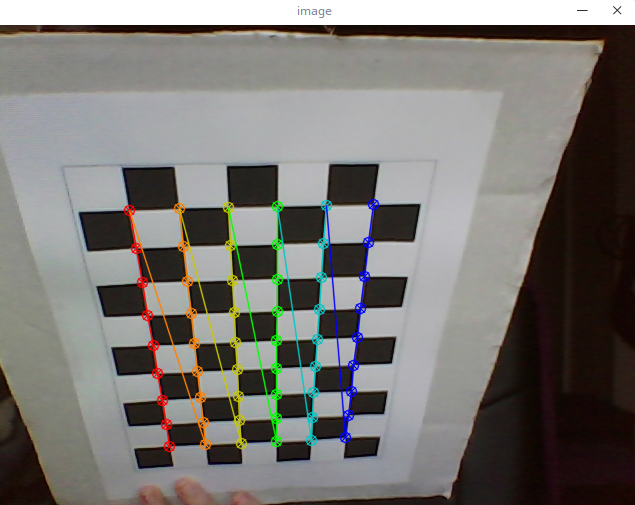
\includegraphics[width=50mm, scale = 0.3]{capitulo_04/figuras_dir/pat6.jpg}}
\subfigure[Posición 7]{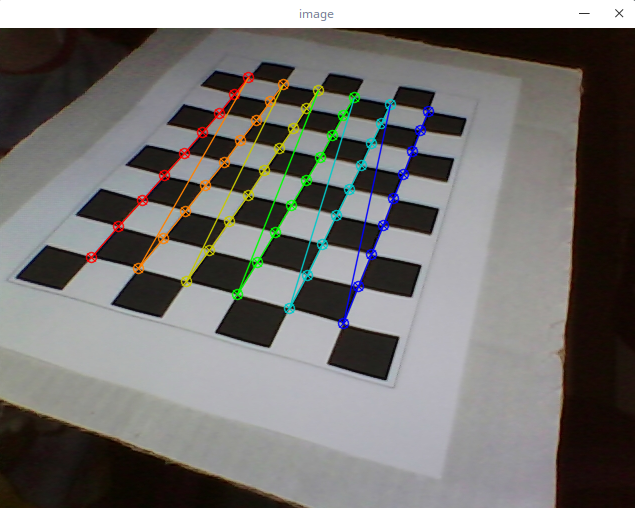
\includegraphics[width=50mm, scale = 0.3]{capitulo_04/figuras_dir/pat7.jpg}}
\subfigure[Posición 8]{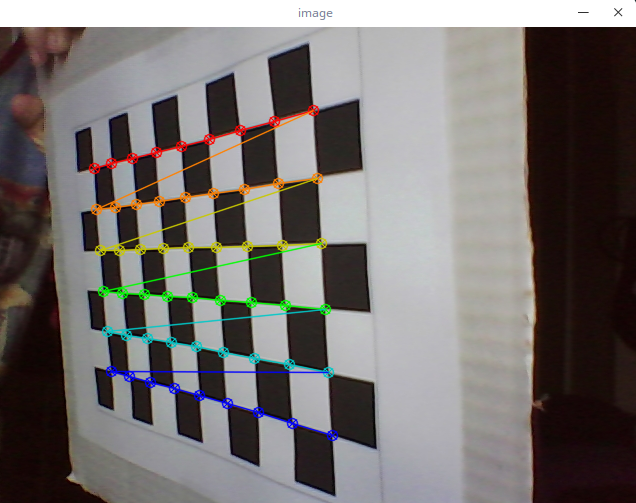
\includegraphics[width=50mm, scale = 0.3]{capitulo_04/figuras_dir/pat8.jpg}}
\subfigure[Posición 9]{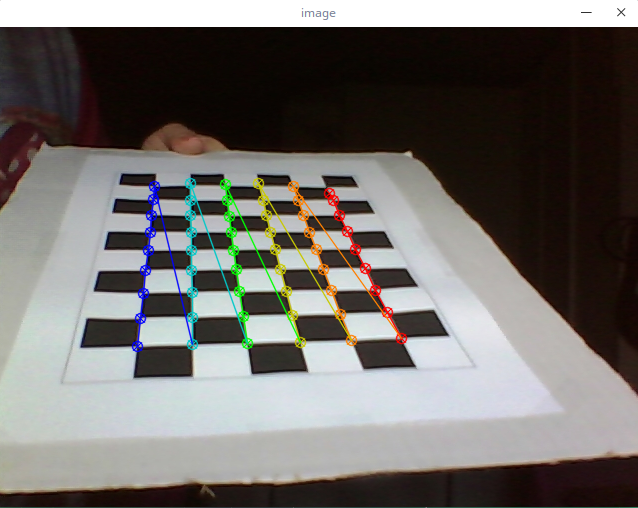
\includegraphics[width=50mm, scale = 0.3]{capitulo_04/figuras_dir/pat9.jpg}}
\subfigure[Posición 10]{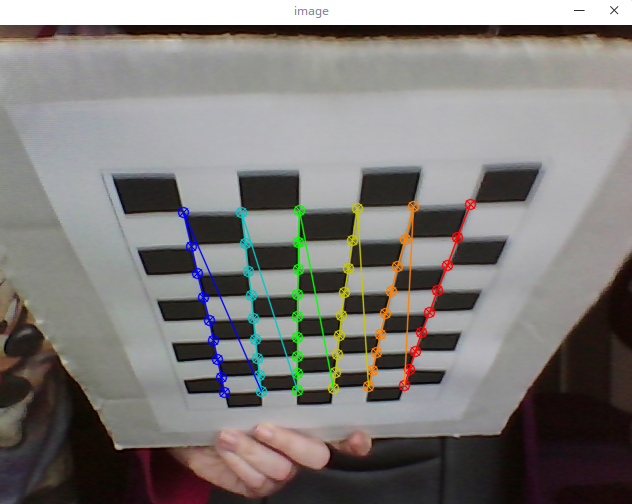
\includegraphics[width=50mm, scale = 0.3]{capitulo_04/figuras_dir/pat10.jpg}}
\subfigure[Posición 11]{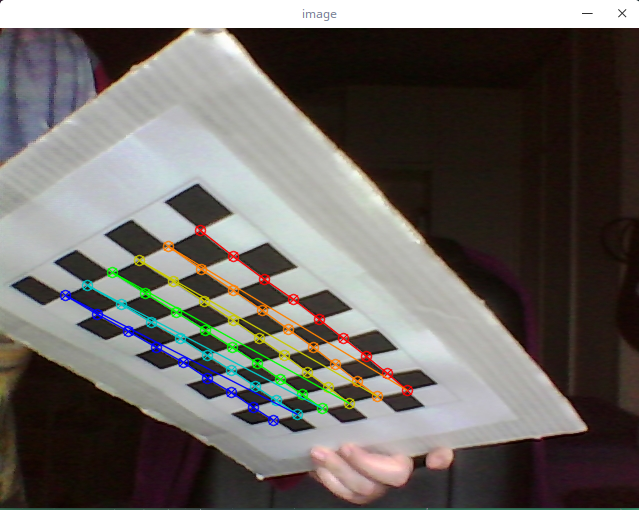
\includegraphics[width=50mm, scale = 0.3]{capitulo_04/figuras_dir/pat11.jpg}}
\subfigure[Posición 12]{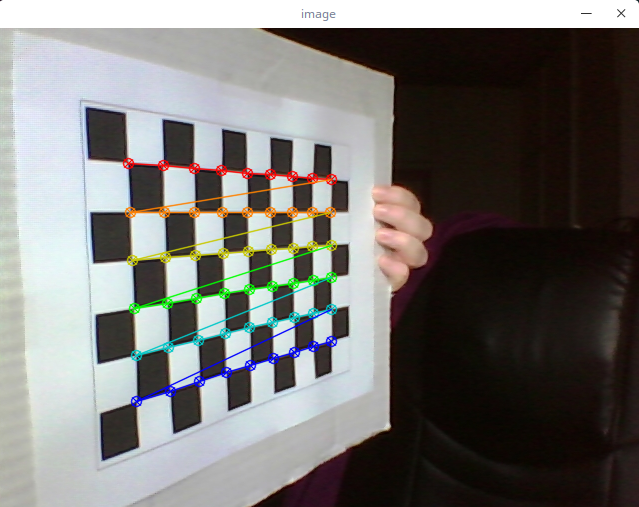
\includegraphics[width=50mm, scale = 0.3]{capitulo_04/figuras_dir/pat12.jpg}}
\subfigure[Posición 13]{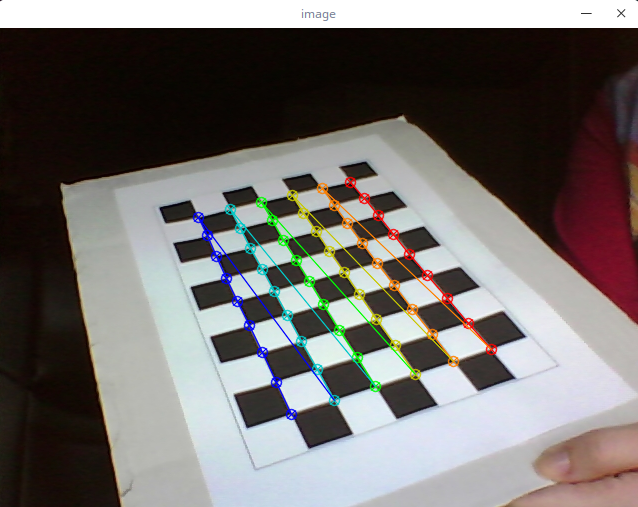
\includegraphics[width=50mm, scale = 0.3]{capitulo_04/figuras_dir/pat13.jpg}}
\subfigure[Posición 14]{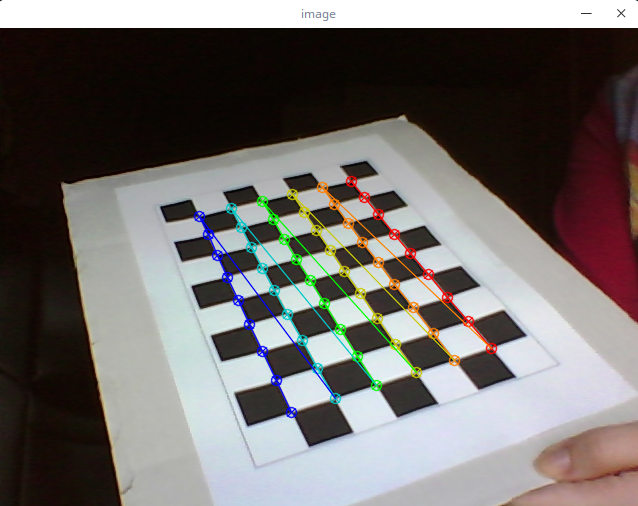
\includegraphics[width=50mm, scale = 0.3]{capitulo_04/figuras_dir/pat14.jpg}}
\caption{Detección del patrón por ``calibration.cpp'' en las imágenes guardadas.} 
%\label{fig:lego}
\end{figure}


    \item Visualización de los valores de los parámetros de la cámara en el terminal: \\

    \begin{figure}
    \centering
    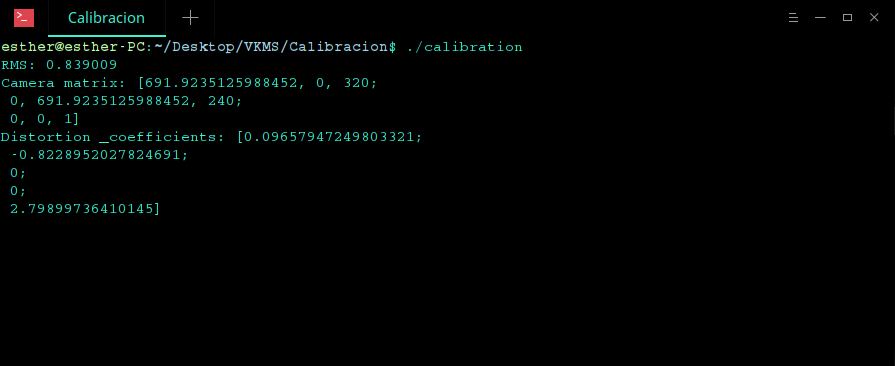
\includegraphics[scale = 0.5]{capitulo_04/figuras_dir/parametros.jpg}
    \caption{Parámetros de la cámara en el terminal}
    %\label{fig:figura4}
    \end{figure}

    \item Archivo de calibración ``MiCam.yml’’: \\
    
    \begin{figure}
    \centering
    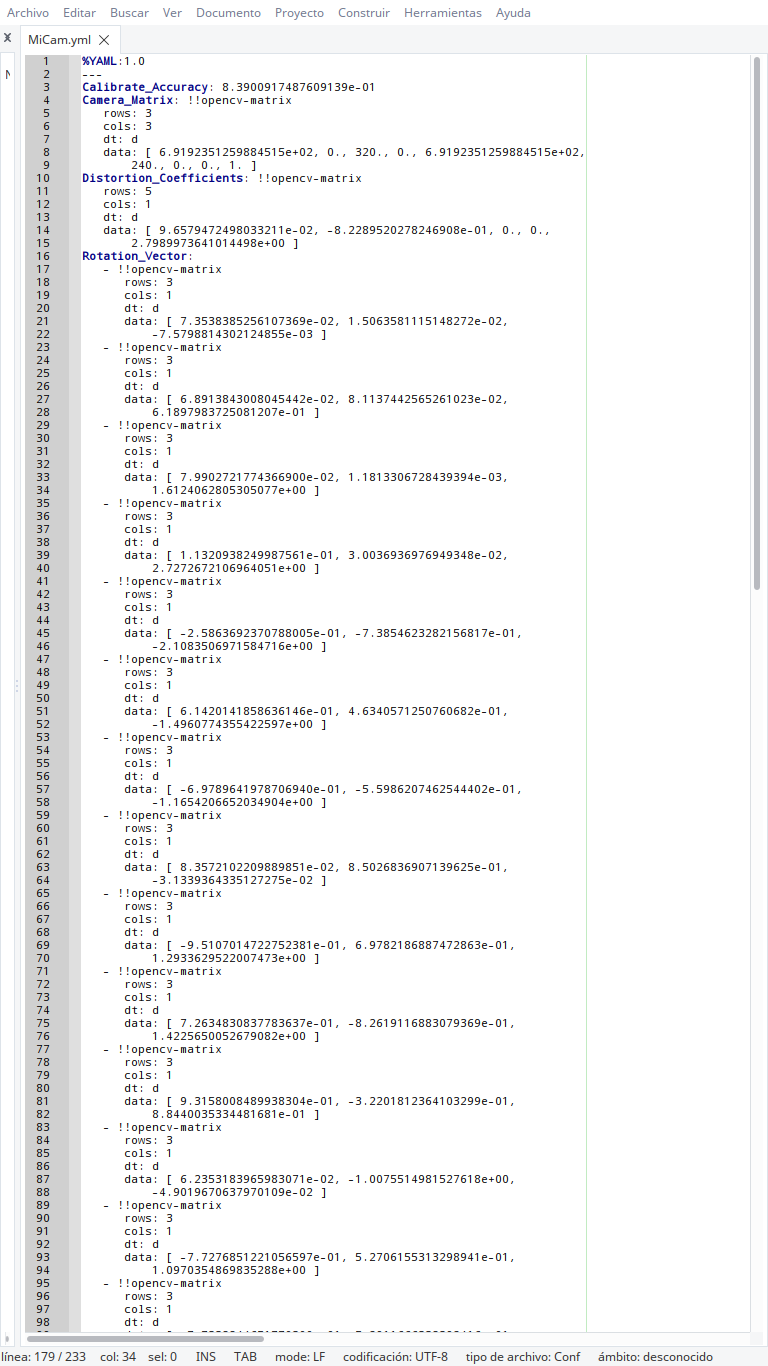
\includegraphics[scale = 0.35]{capitulo_04/figuras_dir/par1.jpg}
    \caption{Número de precisión, matriz de la cámara, coeficientes de distorsión y vector de rotación}
    %\label{fig:figura4}
    \end{figure}
    
    \begin{figure}
    \centering
    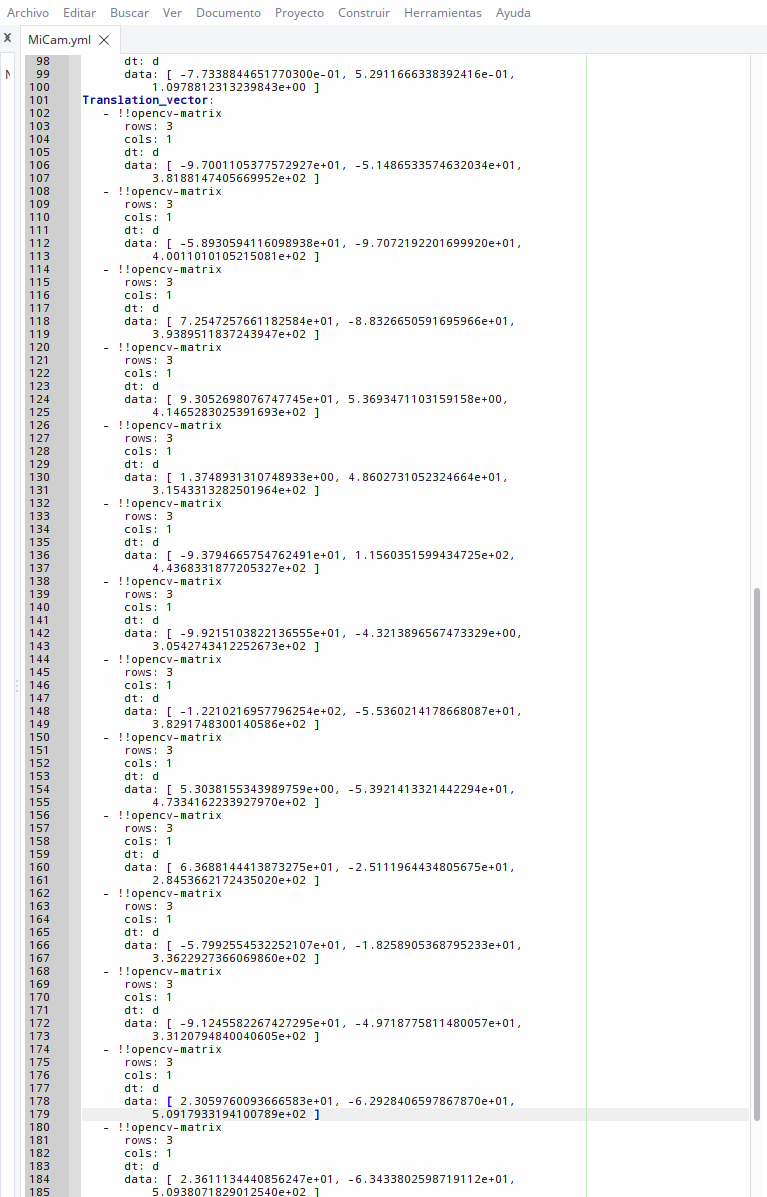
\includegraphics[scale = 0.35]{capitulo_04/figuras_dir/par2.jpg}
    \caption{Vector de traslación}
    %\label{fig:figura4}
    \end{figure}
    
    \begin{figure}
    \centering
    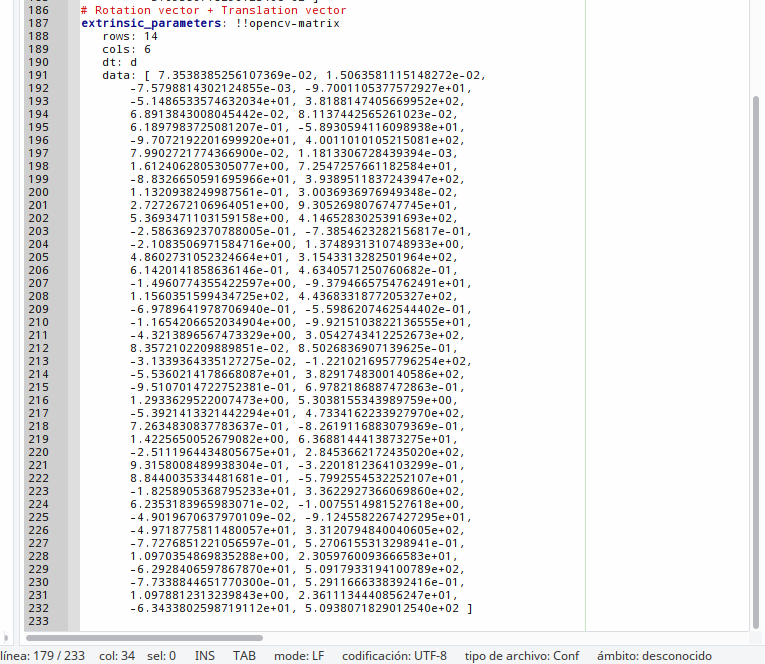
\includegraphics[scale = 0.35]{capitulo_04/figuras_dir/par3.jpg}
    \caption{Concatenación del vector de rotación con el vector de traslación}
    %\label{fig:figura4}
    \end{figure}
    
    \item Imagen real e imagen sin distorsión:
    
\begin{figure}[htbp]
\centering
\subfigure[Imagen distorsionada]{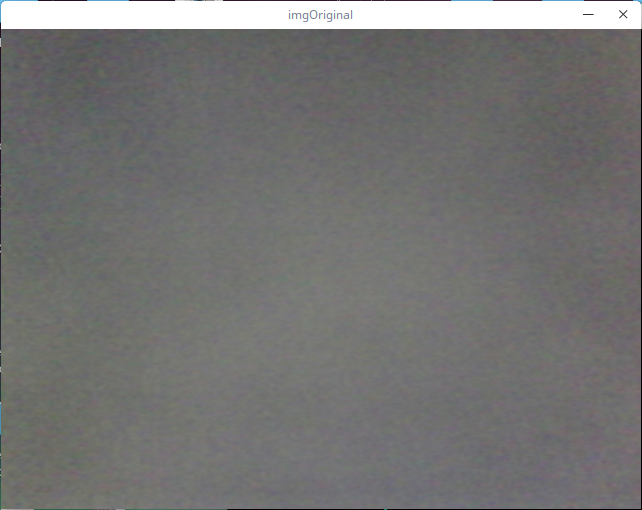
\includegraphics[width=70mm]{capitulo_04/figuras_dir/condist.jpg}}
\subfigure[Imagen sin distorsionar]{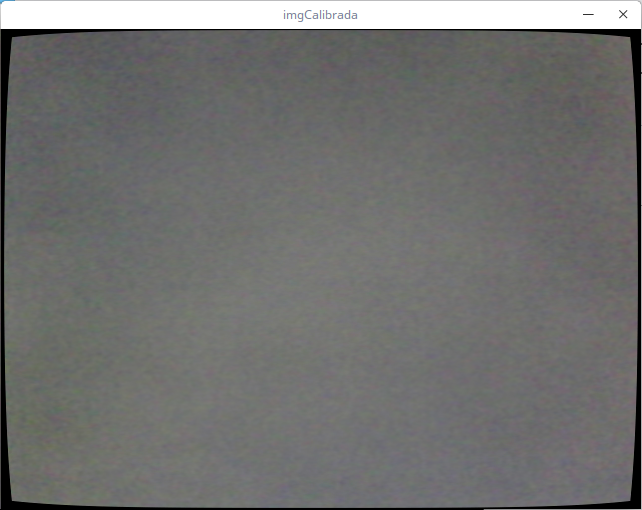
\includegraphics[width=70mm]{capitulo_04/figuras_dir/sindist.jpg}}

\caption{Imagen con y sin distorsión radial} 
\label{fig:sindistorsion}
\end{figure}

\end{itemize}
\end{itemize}


%%%%%%%%%%%%%%%%%%%%%%%%%%%%%%%%%%%%%%%%%%%%%%%%%%%%%%%
%		            	Seccion          			  %
%%%%%%%%%%%%%%%%%%%%%%%%%%%%%%%%%%%%%%%%%%%%%%%%%%%%%%%
\section{Seguimiento ocular con OpenCV} \label{s4_3}


Los parámetros de la cámara son imprecindibles para eliminar la distorsión radial, en concreto, la matriz de la cámara y los coeficientes de distorsión. ``eye\_detect.cpp’’ elimina la distorsión radial cuando llama a la función ``undistort()’’ que carga el archivo que contiene esos parámetros y abre una ventana que muestra las capturas sin distorsión (figura \ref{fig:sindistorsion}). Esto se aprecia en la forma que toman las esquinas de la imagen. En esa ventana, se muestra en cada captura las regiones detectadas con el algoritmo de Viola-Jones (figura \ref{fig:abner}). Estas regiones aparecen delimitadas por recuadros (cara y ojos) y circunferencias (iris). Evidentemente, en este proyecto no interesa la representación de estas zonas, sino que los puntos de la esquina superior izquierda de los recuadros y el centro de la circunferencia en base al ojo izquierdo de la imagen (ojo derecho de la persona). Las coordenadas de estos puntos se reproducen en el terminal. Para diferenciar unos puntos de otros, cada uno viene precedido de una palabra: ``face’’, ``Ojos’’ y ``Pupila’’. Es importante destacar que no todos estos puntos no se toman respecto al sistema de referencia de la imagen cuyo origen es la esquina superior izquierda (O). Sólo el punto del recuadro de la cara (x’, y’) se obtiene respecto O. El punto (x’’, y’’) del recuadro del ojo está medido respecto el recuadro de la cara (O’) y el centro del iris (x’’’, y’’’), respecto el recuadro del ojo (O’’). Para una mejor comprensión del resultado del programa, se representa lo anterior en una imagen aclaratoria:

    \begin{figure}
    \centering
    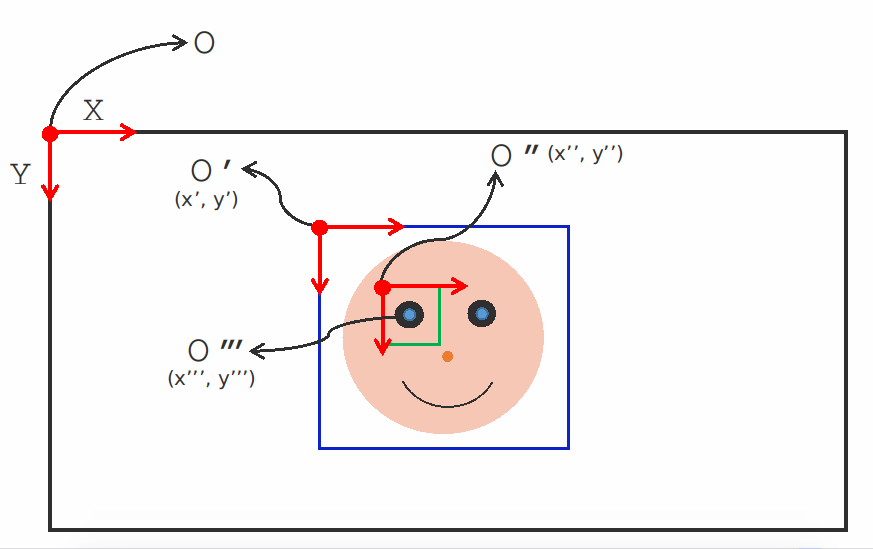
\includegraphics[scale = 0.5]{capitulo_04/figuras_dir/cara.jpg}
    \caption{Representación de los sistemas de referencia}
    %\label{fig:figura4}
    \end{figure}





Como resultado, se obtienen los eventos impresos por pantalla en el terminal:

    \begin{figure}
    \centering
    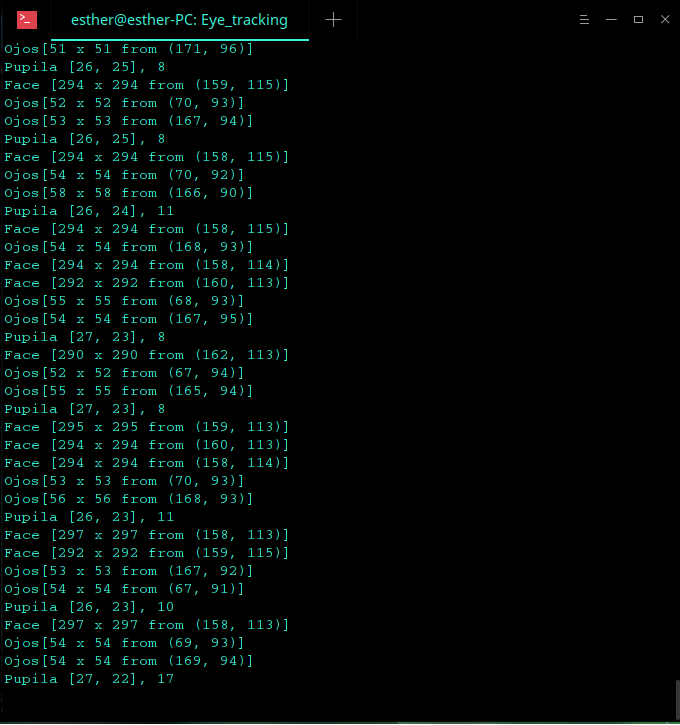
\includegraphics[scale = 0.5]{capitulo_04/figuras_dir/eventos.jpg}
    \caption{Eventos de la cara, ojos y pupila}
    %\label{fig:figura4}
    \end{figure}


%%%%%%%%%%%%%%%%%%%%%%%%%%%%%%%%%%%%%%%%%%%%%%%%%%%%%%%
%		            	Seccion          			  %
%%%%%%%%%%%%%%%%%%%%%%%%%%%%%%%%%%%%%%%%%%%%%%%%%%%%%%%
\section{Comunicación Raspberry Pi - Arduino} \label{s4_4}

%%%%%%%%%%%%%%%%%%%%% Subsección %%%%%%%%%%%%%%%%%%%%%
\subsection{Instalación de Arduino IDE} \label{s4_4_1}

Arduino IDE es el software oficial de Arduino que incorpora la interfaz de programación y todas las bibliotecas necesarias en la compilación de varios tipos de programas. En este proyecto, se usa para compilar y cargar el programa ``Servidor\_TCP.ino'' y así, iniciar el servidor de la comunicación Raspberry Pi Zero - Arduino.

Para instalarlo, en primer lugar hay que descargarlo en la página oficial a través de la siguiente dirección: ``http://www.arduino.cc/en/Main/Software''. Debajo del título ``Download the Arduino IDE'' se selecciona la versión del sistema operativo y comienza la descarga de un archivo de formato ``.zip'' automáticamente. El siguiente paso, consiste en descomprimir el archivo y establecer como directorio de trabajo la carpeta resultante de la descomposición mediante el comando ``cd'' en el terminal. Posteriormente, se teclea la orden: \\

\begin{bashcode}
$ ./install.sh
\end{bashcode}

Tras esto, la instalación se ha completado pero puede que se produzcan errorres al subir el archivo por el puerto correspondiente. Esto sucede debido a que no se han establecido los permisos del puerto serie. Para visualizar los permisos se introduce en el terminal: \\

\begin{bashcode}
$ ls -l /dev/ttyACM*
\end{bashcode}

Esta orden permite informar sobre los permisos de todos los puertos ``ttyACM'' con independencia de su enumeración.
Para resolver el problema anterior, se añade el usuario propio al grupo de la siguiente forma:

\begin{bashcode}
$ sudo usermod -a -G dialout <nombreusuario>
\end{bashcode}


\subsection{Resultados de la comunicación} \label{s4_4_2}

Para observar cómo se reciben los eventos, es necesario ejecutar todos los programas elaborados hasta ahora: ``mk.c'', ``eye\_detect.cpp'', ``Selector.c'', ``Cliente.c'' y ``Servidor\_TCP.ino'' como se muestra en la figura \ref{fig:programas}.


\begin{figure}[htbp]
\centering
\subfigure[Ejecución de ``mk.c'']{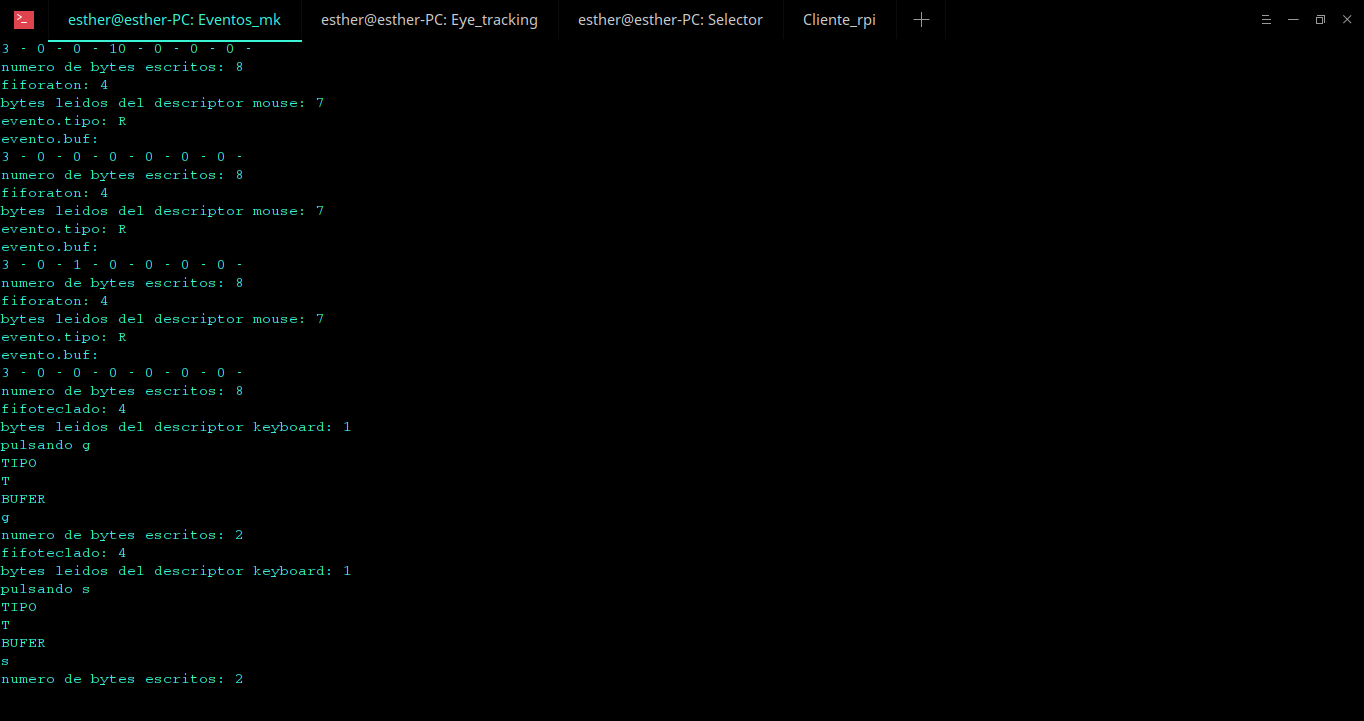
\includegraphics[width=80mm]{capitulo_04/figuras_dir/abrirmk.jpg}}
\subfigure[Ejecución de ``eye\_detect.cpp'']{\includegraphics[width=80mm]{capitulo_04/figuras_dir/abrireye_tracking.jpg}}
\subfigure[Ejecución de ``Selector.c'']{\includegraphics[width=80mm]{capitulo_04/figuras_dir/abrirselector.jpg}}
\subfigure[Ejecución de ``Cliente.c'']{\includegraphics[width=80mm]{capitulo_04/figuras_dir/abrircliente.jpg}}

\label{fig:programas}
\end{figure}

A continuación, se muestran los eventos representados en hexadecimal por el programa ``mk.c'' y la recepción de los mismos por el servidor Arduino.

    \begin{figure}
    \centering
    \includegraphics[scale = 0.5]{capitulo_04/figuras_dir/clickder2.jpg}
    \caption{``Click'' derecho.}
    %\label{fig:figura4}
    \end{figure}

    \begin{figure}
    \centering
    \includegraphics[scale = 0.5]{capitulo_04/figuras_dir/clickizq2.jpg}
    \caption{``Click'' izquierdo.}
    %\label{fig:figura4}
    \end{figure}

    \begin{figure}
    \centering
    \includegraphics[scale = 0.5]{capitulo_04/figuras_dir/movx+.jpg}
    \caption{Movimiento en sentido positivo del eje X.}
    %\label{fig:figura4}
    \end{figure}

    \begin{figure}
    \centering
    \includegraphics[scale = 0.5]{capitulo_04/figuras_dir/movx-.jpg}
    \caption{Movimiento en sentido negativo del eje X.}
    %\label{fig:figura4}
    \end{figure}

    \begin{figure}
    \centering
    \includegraphics[scale = 0.5]{capitulo_04/figuras_dir/movy+.jpg}
    \caption{Movimiento en sentido positivo del eje Y.}
    %\label{fig:figura4}
    \end{figure}

    \begin{figure}
    \centering
    \includegraphics[scale = 0.5]{capitulo_04/figuras_dir/movy-.jpg}
    \caption{Movimiento en sentido positivo del eje Y.}
    %\label{fig:figura4}
    \end{figure}

    \begin{figure}
    \centering
    \includegraphics[scale = 0.5]{capitulo_04/figuras_dir/teclau.jpg}
    \caption{Pulsación de la tecla ``u''.}
    %\label{fig:figura4}
    \end{figure}


%%%%%%%%%%%%%%%%%%%%%%%%%%%%%%%%%%%%%%%%%%%%%%%%%%%%%%%
%		            	Seccion          			  %
%%%%%%%%%%%%%%%%%%%%%%%%%%%%%%%%%%%%%%%%%%%%%%%%%%%%%%%
\section{Programa de selección} \label{s4_5}

El programa ``selector.c'' descrito en la sección 3.4, permite determinar el lugar hacia donde mira el observador analizando y comparando el valor de la coordenada x'' (coordenada x del evento del ojo) en relación a dos valores: ``x1'' y ``x2''. Cada uno de ellos constituye un límite en el eje de abscisas. Cuando el observador mira hacia la derecha fuera de la pantalla principal, el valor de x'' es igual o superior a ``x2'', en ese momento, ``selector.c'' envía ``B''. Cuando mira hacia la izquierda fuera de la pantalla, x'' es igual o inferior a ``x1'', momento en el que también se envía ``B'' al cliente, ya que cualquier cambio hacia una pantalla secundaria, se indica con este caracter al programa cliente. 

Estos valores límite se obtienen tras sucesivas pruebas. En primer lugar, se ejecuta ``eye\_detect.cpp'' para guardar los eventos en FIFO y posteriormente, ``selector.c'' que recoge todos esos datos escritos mediante operaciones de lectura y realiza la media de las coordenadas x de cinco eventos de ojos sucesivos (precedidos por el tipo ``E'').

A continuación, se exponen los valores de esta coordenada cuando el observador mira a la pantalla principal (vista frente), a una pantalla secundaria situada a la derecha de la principal (vista derecha) y a una pantalla secundaria situada a la izquierda de la principal (vista izquierda):


\begin{longtable}{c|c|c|c}
    %\centering
    \caption{Valores de x'' en función de la dirección de la mirada} \\
     Número de muestra & Vista frente & Vista derecha & Vista izquierda \\ \hline
     \endfirsthead
     \caption{Continuación} \\
     Número de muestra & Vista frente & Vista derecha & Vista izquierda \\ \hline
     \endhead
    \multicolumn{4}{c}{(Sigue en la página siguiente)} \\   
     \endfoot
     \multicolumn{4}{c}{(Fin de la tabla)} \\
     \endlastfoot
     0 & 47 & 50 & 43 \\
     1 & 48 & 59 & 42 \\
     2 & 48 & 59 & 42 \\
     3 & 50 & 60 & 43 \\
     4 & 51 & 59 & 42 \\
     5 & 48 & 59 & 41 \\
     6 & 47 & 62 & 42 \\
     7 & 48 & 60 & 42 \\
     8 & 50 & 61 & 40 \\
     9 & 48 & 59 & 42 \\
     10 & 49 & 61 & 43 \\
     11 & 49 & 60 & 43 \\
     12 & 48 & 60 & 43 \\
     13 & 46 & 59 & 44 \\
     14 & 48 & 62 & 42 \\
     15 & 48 & 60 & 40 \\
     16 & 49 & 59 & 41 \\
     17 & 51 & 61 & 42 \\
     18 & 50 & 60 & 42 \\
     19 & 49 & 62 & 43 \\
     20 & 47 & 61 & 43 \\
     21 & 48 & 62 & 44 \\
     22 & 48 & 63 & 44 \\
     23 & 47 & 60 & 43 \\
     24 & 46 & 59 & 42 \\
     25 & 47 & 59 & 42 \\
     26 & 45 & 61 & 43 \\
     27 & 48 & 59 & 42 \\
     28 & 48 & 59 & 43 \\
     29 & 49 & 60 & 44 \\
     30 & 48 & 59 & 43 \\ 
     31 & 49 & 61 & 41 \\ 
     32 & 48 & 61 & 42 \\ 
     33 & 50 & 60 & 44 \\ 
     34 & 51 & 62 & 43 \\ 
     35 & 51 & 59 & 43 \\ 
     36 & 50 & 61 & 43 \\ 
     37 & 49 & 63 & 43 \\ 
     38 & 48 & 60 & 43 \\ 
     39 & 48 & 59 & 44 \\ 
     40 & 50 & 59 & 41 \\ 
     41 & 48 & 60 & 42 \\ 
     42 & 47 & 59 & 42 \\ 
     43 & 47 & 59 & 43 \\ 
     44 & 45 & 61 & 43 \\ 
     45 & 50 & 59 & 44 \\ 
     46 & 48 & 60 & 43 \\ 
     47 & 47 & 60 & 44 \\ 
     48 & 47 & 59 & 42 \\ 
     49 & 48 & 62 & 41 \\ 
     50 & 49 & 61 & 43 \\ \hline
\end{longtable}

Se observa que cuando el observador mira a la pantalla principal, los valores de x'' oscilan entre 45 y 51, cuando mira a la derecha de ésta, entre 59 y 63 y cuando mira a la izquierda de ésta, entre 40 y 44. Por tanto, puede establecerse como límite superior (``x2'') un valor de 59 y como límite inferior, un valor de 44 (``x2'') tendiendo en cuenta que 59 es el mínimo valor de x'' cuando el observador mira a la derecha y 44, el valor máximo de x'' cuando el observador mira a la izquierda.

Todo lo que se expone a continuación está referido a lo que el observador ve al mirar la pantalla del monitor como todo lo que se lleva explicando hasta ahora. Es importante saber que todo lo que el observador tiene a su izquierda, se representa en la imagen capturada por la cámara en el lado de la derecha y viceversa. 

Se concluye con datos numéricos anteriores y con las regiones dibujadas que, cuando se inclina la cabeza hacia la derecha (en la imagen capturada por la cámara que se muestra en la pantalla se visualiza el movimiento en la izquierda), el marco de la cara se aproxima al lado más visible de ésta (quedando parte de ella oculta). Es lo mismo que decir que el lado derecho del cuadro facial se acerca a la derecha de la cara. De esto se deduce que O'' se encuentra más lejos de O' ya que en la imagen el cuadrado del ojo izquierdo se encuentra más alejado de O' por haberse movido éste hacia el mismo lado. Sucede lo mismo cuando el observador gira la cabeza hacia la izquierda. En este último caso, el lado izquierdo del cuadrado facial se aproxima al lado izquierdo de la cara y por ende, O' y O'' están más próximos entre sí.

Abner Matheus \citep{eyetracking} implementó el programa de seguimiento ocular con el objetivo de crear un sistema de control del ratón y lo mostró en un vídeo. Dado que ``eye\_detect.cpp'' es la parte de su programa encargada de la detección, funciona de la misma manera que él muestra (figura \ref{fig:abner}).

\begin{figure}[htbp]
\centering
\subfigure[Giro hacia de la cabeza hacia la derecha]{\includegraphics[width=50mm]{capitulo_04/figuras_dir/Der.jpg}}
\subfigure[Giro de la cabeza hacia la izquierda]{\includegraphics[width=50mm, scale = 0.3]{capitulo_04/figuras_dir/Izq.jpg}}
\subfigure[Cabeza en posición frontal]{\includegraphics[width=50mm, scale = 0.3]{capitulo_04/figuras_dir/frente.jpg}}
\caption{Capturas tomadas a partir del vídeo de Abner Matheus.} 
\label{fig:abner}
\end{figure}

Las tres imágenes anteriores ayudan a comprender los datos obtenidos en la tabla anterior. Como se ha mencionado, cuando se mira hacia la derecha, con el movimiento de cabeza que conlleva, el lado izquierdo del cuadro azul (región facial) se aleja del lado izquierdo del cuadrado verde izquierdo y por tanto, mayor es x''. Cuando el observador gira la cabeza hacia la izquierda, el lado izquierdo del cuadrado azul se acerca al lado izquierdo del cuadrado verde izquierdo y por tanto, menor es x''. Sin embargo, con la cabeza en posición frontal, el cuadrado azul mantiene centrados ambos cuadrados verdes y x'' toma un valor intermedio entre los dos anteriores. \\ \\

Los elementos anteriores sirven para determinar ``x1'' y ``x2''. Cuando a cada variable se le asigna su valor, lo único que falta es comprobar si el programa filtra los eventos correctamente y si envía al cliente la variable adecuada. A continuación, se representa la salida del programa de detección y del programa de selección cuando éste está configurado con la pantalla secundaria a la izquierda y el usuario mira a la pantalla y a ambos lados:

    \begin{figure}
    \centering
    \includegraphics[scale = 0.4]{capitulo_04/figuras_dir/ldcentro.jpg}
    \caption{Vista al frente}
    %\label{fig:figura4}
    \end{figure}

    \begin{figure}
    \centering
    \includegraphics[scale = 0.4]{capitulo_04/figuras_dir/ldder.jpg}
    \caption{Vista a la derecha}
    %\label{fig:figura4}
    \end{figure}

    \begin{figure}
    \centering
    \includegraphics[scale = 0.4]{capitulo_04/figuras_dir/ldizq.jpg}
    \caption{Vista a la izquierda}
    %\label{fig:figura4}
    \end{figure}


El programa ``selector.c'' muestra entre corchetes las dimensiones del cuadrado que limita la región ocular y entre paréntesis, las coordenadas de los eventos de los ojos, ignorando los de la pupila que en este caso no son necesarios. 


%%%%%%%%%%%%%%%%%%%%%%%%%%%%%%%%%%%%%%%%%%%%%%%%%%%%%%%
%		            	Seccion          			  %
%%%%%%%%%%%%%%%%%%%%%%%%%%%%%%%%%%%%%%%%%%%%%%%%%%%%%%%
\section{Simulación de teclas en Arduino} \label{s4_6}

Para la simulación de teclas, se procede a montar un pequeño circuito consistente en interruptores que comunican las entradas ``0'' y ``1'' de Arduino Leonardo a tierra. Para demostrar el funcionamiento de la simulación de teclas, se usa el código siguiente. En él, se asignan los pines anteriores como entradas ``pull up'', es decir, se las puede dar un valor de 0 lógico derivando su señal a tierra mediante un pulsador. En ese momento, se detecta que el botón correspondiente a uno de los pines es accionado, y se llama a ``keyboard.write()''. En el caso de pulsarse el interruptor correspondiente al pin 0, se escribe una ``A'' y en caso de que sea el correspondiente al pin 1, se escribe una frase completa. Si el cursor se sitúa en un documento Word o Libre Office, el resultado es como el que se muestra en la figura \ref{fig:simteclas}.



\begin{listing}
\begin{minted}[bgcolor=bg,
               frame=lines,
               framesep=2mm,
               linenos]
               {C}

#include <Keyboard.h> 

void setup() {
    pinMode(0,INPUT_PULLUP);  
    pinMode(1,INPUT_PULLUP);  
    
    Serial.begin(9600);   

}

void loop() {
  
     Keyboard.begin();       
     if (digitalRead(0) == 0)  
      {
        Keyboard.write('A');  
        delay(200);           
      }
      else if (digitalRead(1) == 0){  
        Keyboard.print("The rain in Spain falls mainly on the plain"); 
        delay(200);
    }
      Keyboard.end();                
}
\end{minted}
\caption{Código de muestra para la simulación de teclas.}
\label{Listing}
\end{listing}

    \begin{figure}
    \centering
    \includegraphics[scale = 0.07]{capitulo_04/figuras_dir/montsim.jpg}
    \caption{Montaje de la simulación}
    \label{fig:simteclas}
    \end{figure}



    \begin{figure}
    \centering
    \includegraphics[scale = 0.3]{capitulo_04/figuras_dir/simteclas.jpg}
    \caption{Resultado de la simulación}
    \label{fig:simteclas}
    \end{figure}










%%%%%%%%%%%%%%%%%%%%%%%%%%%%%%%%%%%%%%%%%%%%%%%%%%%%%%%
%		            	Seccion          			  %
%%%%%%%%%%%%%%%%%%%%%%%%%%%%%%%%%%%%%%%%%%%%%%%%%%%%%%%
%\section{Resultado final} \label{s4_7}

